\documentclass[12pt,a4paper]{article}

% ──────────────────────────────────────────────
% Packages
% ──────────────────────────────────────────────
\usepackage[utf8]{inputenc}
\usepackage[T1]{fontenc}
\usepackage[french]{babel}
\usepackage{amsmath,amssymb,amsthm}
\usepackage{graphicx}
\graphicspath{{figures/}}
\usepackage{booktabs}
\usepackage{caption}
\usepackage{subcaption}
\usepackage[margin=2.5cm]{geometry}
\usepackage{hyperref}

\usepackage{natbib}
\usepackage{enumitem}
\usepackage{float}
\usepackage{array}
\usepackage{multirow}
\usepackage{xcolor}
\usepackage{setspace}

\onehalfspacing

\hypersetup{
    colorlinks=true,
    linkcolor=blue!60!black,
    citecolor=blue!60!black,
    urlcolor=blue!60!black
}

% ──────────────────────────────────────────────
% Commandes personnalisées
% ──────────────────────────────────────────────
\newcommand{\R}{\mathbb{R}}
\newcommand{\N}{\mathbb{N}}
\DeclareMathOperator*{\argmin}{arg\,min}

% ──────────────────────────────────────────────
% Page de titre
% ──────────────────────────────────────────────
\title{%
    \vspace{-1cm}
    \textsc{ENSAE Paris} \\[0.3cm]
    \textsc{Projet Stat'App} \\[0.8cm]
    \rule{\linewidth}{0.5mm} \\[0.4cm]
    {\LARGE \textbf{Segmentation automatique de lésions cutanées \\[0.2cm]
    en imagerie dermoscopique : \\[0.2cm]
    des méthodes classiques à l'apprentissage profond}} \\[0.3cm]
    \rule{\linewidth}{0.5mm} \\[0.6cm]
    {\large Sous la direction d'Aline Helburg --- Headmind Partners}
}

\author{
    Louis \textsc{Maurice} \and
    Ziad \textsc{Dira} \and
    Mehdi \textsc{Sfar} \and
    Clément \textsc{Hadji}
}

\date{Mars 2026}

\begin{document}

\maketitle
\thispagestyle{empty}
\newpage

% ──────────────────────────────────────────────
% Résumé / Abstract
% ──────────────────────────────────────────────
\begin{abstract}
La segmentation automatique de lésions cutanées en imagerie dermoscopique constitue une étape clé de l'aide au diagnostic du mélanome. Ce travail explore, implémente et compare trois approches de complexité croissante sur le jeu de données ISIC~2016 (900~images d'entraînement, 379~images de test)~: (i)~une segmentation non supervisée par $K$-means, évaluée dans quatre espaces colorimétriques avec étude d'ablation sur le nombre de clusters et la règle d'assignation~; (ii)~un CNN par patches, introduisant convolutions apprises et supervision comme étape intermédiaire~; (iii)~une architecture U-Net, optimisée par une étude d'ablation systématique portant sur 13~axes d'hyperparamètres (24~expériences). La progression des performances suit la complexité des modèles~: le $K$-means LAB atteint un coefficient de Dice (DSC) de $0{,}648$ sur le jeu de test, le CNN par patches $0{,}760$ ($+0{,}112$), et le U-Net final $0{,}882$ ($+0{,}122$), soit un indice de Jaccard de $0{,}807$ --- un résultat compétitif par rapport aux participants du challenge ISBI~2016. L'analyse par sous-groupes de difficulté et les tests de significativité statistique confirment la supériorité des approches supervisées, en particulier pour les petites lésions et les cas à faible contraste.
\end{abstract}

\paragraph*{Mots-clés.} Segmentation d'images médicales, dermoscopie, lésions cutanées, $K$-means, réseau de neurones convolutif, U-Net, étude d'ablation, ISIC~2016.

\vspace{1cm}

\begin{abstract}
\selectlanguage{english}
Automatic segmentation of skin lesions in dermoscopic images is a key step in computer-aided melanoma diagnosis. This work explores, implements, and compares three approaches of increasing complexity on the ISIC~2016 dataset (900~training images, 379~test images): (i)~unsupervised $K$-means segmentation, evaluated across four colour spaces with ablation on the number of clusters and assignment rule; (ii)~a patch-based CNN, introducing learned convolutions and supervision as an intermediate step; (iii)~a U-Net architecture, optimised through a systematic ablation study spanning 13~hyperparameter axes (24~experiments). Performance tracks model complexity: the LAB $K$-means achieves a Dice coefficient (DSC) of $0.648$ on the test set, the patch CNN $0.760$ ($+0.112$), and the final U-Net $0.882$ ($+0.122$), yielding a Jaccard index of $0.807$ --- competitive with the ISBI~2016 challenge participants. Subgroup analysis by difficulty and paired statistical tests confirm the superiority of supervised methods, especially for small lesions and low-contrast cases.
\selectlanguage{french}
\end{abstract}

\paragraph*{Keywords.} Medical image segmentation, dermoscopy, skin lesions, $K$-means, convolutional neural network, U-Net, ablation study, ISIC~2016.

\newpage

% ──────────────────────────────────────────────
% Table des matières
% ──────────────────────────────────────────────
\tableofcontents
\newpage

% ══════════════════════════════════════════════
% 1. INTRODUCTION
% ══════════════════════════════════════════════
\section{Introduction}

\subsection{Contexte}

L'imagerie médicale constitue un pilier fondamental de la médecine contemporaine, intervenant à chaque étape du parcours clinique~: diagnostic, suivi thérapeutique et planification des interventions. Parmi les tâches d'analyse d'images, la \emph{segmentation} --- c'est-à-dire la délimitation automatique de régions d'intérêt (organes, tumeurs, lésions) au sein d'une image --- occupe une place centrale. En radiothérapie, par exemple, une segmentation précise des tumeurs et des tissus sains adjacents conditionne directement la qualité du plan de traitement et, \emph{in fine}, le pronostic du patient \citep{hesamian2019deep}.

Dans le domaine dermatologique, la dermoscopie a considérablement amélioré l'examen visuel des lésions cutanées pigmentées, permettant une observation à fort grossissement des structures morphologiques sous-cutanées. Toutefois, l'analyse des images dermoscopiques demeure une procédure majoritairement manuelle, longue, sujette à la variabilité inter-opérateur et fortement dépendante de l'expertise du clinicien \citep{codella2018skin}. Or, le cancer de la peau --- et en particulier le mélanome --- représente l'un des cancers dont l'incidence croît le plus rapidement dans les pays industrialisés. La détection précoce, facilitée par une segmentation fiable des lésions, constitue un levier majeur de réduction de la mortalité.

\subsection{Problématique}

La segmentation automatique de lésions cutanées en imagerie dermoscopique se heurte à plusieurs défis~:
\begin{itemize}[nosep]
    \item le \textbf{faible contraste} entre la lésion et la peau environnante dans certaines configurations (lésions hypopigmentées, peaux claires)~;
    \item la \textbf{variabilité morphologique} des lésions (taille, forme, texture, couleur)~;
    \item la présence d'\textbf{artefacts} (poils, bulles d'air, reflets spéculaires, marquages cliniques) qui perturbent les contours~;
    \item l'\textbf{hétérogénéité} des conditions d'acquisition (résolution, éclairage, dispositif optique).
\end{itemize}

Ces difficultés motivent le développement de méthodes automatiques robustes, capables de produire des masques de segmentation de qualité clinique tout en étant suffisamment généralisables pour traiter des images acquises dans des conditions variées.

\subsection{Objectifs du projet}

Ce projet vise à explorer, implémenter et comparer différentes approches de segmentation de lésions cutanées, en progressant des méthodes les plus simples vers les plus sophistiquées~:
\begin{enumerate}[nosep]
    \item \textbf{Analyse exploratoire approfondie} du jeu de données ISIC~2016, afin de caractériser les propriétés géométriques, topologiques et photométriques des images et des masques de référence, et d'en déduire les contraintes de modélisation.
    \item \textbf{Implémentation de méthodes classiques} de segmentation non supervisée, en particulier l'algorithme des $K$-means appliqué dans l'espace colorimétrique, afin d'établir une ligne de base (\emph{baseline}).
    \item \textbf{Mise en \oe uvre d'approches supervisées de complexité croissante}~: un CNN par patches, introduisant convolutions apprises et supervision comme étape intermédiaire, puis une architecture U-Net \citep{ronneberger2015unet} optimisée par étude d'ablation systématique.
    \item \textbf{Évaluation rigoureuse et comparative} des modèles à l'aide de métriques standard (coefficient de Dice, \emph{Intersection over Union}, précision, rappel), incluant une analyse par sous-groupes de difficulté et des tests de significativité statistique.
\end{enumerate}

\subsection{Contributions}

Les contributions principales de ce travail sont les suivantes~:
\begin{enumerate}[nosep]
    \item Une \textbf{analyse exploratoire systématique} du jeu de données ISIC~2016, couvrant cinq axes (géométrie, taille des lésions, topologie, localisation spatiale, contraste photométrique) et leurs implications méthodologiques.
    \item Une \textbf{évaluation exhaustive du $K$-means} comme baseline non supervisée~: quatre espaces colorimétriques, trois méthodes d'estimation du $K$ optimal, deux règles d'assignation, avec analyse par sous-groupes de difficulté.
    \item L'introduction d'un \textbf{CNN par patches comme étape intermédiaire}, permettant d'isoler les contributions respectives des convolutions apprises, de la supervision et du contexte global.
    \item Une \textbf{étude d'ablation systématique} du U-Net portant sur 13 axes d'hyperparamètres (24~expériences), aboutissant à un modèle final compétitif avec les résultats du challenge ISBI~2016 (DSC~$= 0{,}882$, Jaccard~$= 0{,}807$).
\end{enumerate}

\subsection{Organisation du document}

La suite de ce document est organisée comme suit. La section~\ref{sec:revue} présente une revue de la littérature sur la segmentation d'images médicales. La section~\ref{sec:donnees} décrit en détail le jeu de données ISIC~2016 et les résultats de l'analyse exploratoire. La section~\ref{sec:methodologie} formalise le problème de segmentation et détaille les méthodes employées, incluant le protocole d'entraînement et la stratégie d'étude d'ablation. La section~\ref{sec:resultats} présente l'ensemble des résultats expérimentaux~: évaluation comparative du $K$-means dans quatre espaces colorimétriques et étude d'ablation sur le choix de $K$ et la règle d'assignation, puis évaluation d'un CNN par patches comme approche intermédiaire supervisée, et enfin étude d'ablation systématique de l'architecture U-Net sur 13 axes d'hyperparamètres et évaluation du modèle final optimisé, incluant une comparaison par sous-groupes de difficulté et un positionnement par rapport au challenge ISBI~2016. La section~\ref{sec:conclusion} dresse le bilan du projet et la section~\ref{sec:perspectives} trace les axes d'approfondissement envisagés.


% ══════════════════════════════════════════════
% 2. REVUE DE LITTÉRATURE
% ══════════════════════════════════════════════
\section{Revue de littérature}
\label{sec:revue}

\subsection{Approches classiques de segmentation}

Les premières méthodes de segmentation d'images médicales reposent sur des approches dites \emph{classiques}, que l'on peut regrouper en trois grandes familles~:

\paragraph{Méthodes par seuillage.} Le seuillage consiste à partitionner les pixels d'une image en fonction de leur intensité, en définissant un ou plusieurs seuils. La méthode d'Otsu \citep{otsu1979threshold}, qui maximise la variance inter-classes, en constitue un exemple canonique. Bien que simple et efficace lorsque le contraste est élevé, le seuillage échoue face aux images dermoscopiques présentant un faible contraste lésion/fond ou des artefacts d'illumination.

\paragraph{Méthodes par clustering.} Les algorithmes de partitionnement non supervisé, tels que $K$-means \citep{macqueen1967kmeans} ou les modèles de mélange gaussien (GMM), regroupent les pixels dans un espace de caractéristiques (typiquement l'espace colorimétrique RGB ou LAB) sans nécessiter d'annotations. Si ces approches offrent une flexibilité appréciable, elles restent sensibles à l'initialisation, ne modélisent pas la structure spatiale de l'image et sont vulnérables aux artefacts (poils, reflets) qui perturbent la distribution des intensités.

\paragraph{Modèles déformables et contours actifs.} Les \emph{snakes} \citep{kass1988snakes} et les \emph{level sets} propagent un contour initial vers les frontières de l'objet en minimisant une fonctionnelle d'énergie. Ces méthodes intègrent des a priori géométriques (régularité, courbure), mais sont sensibles à l'initialisation et convergent difficilement en présence de contours faibles ou bruités.

Ces approches classiques, bien qu'utiles comme références de base, présentent des limites structurelles~: elles n'exploitent pas --- ou très peu --- le contexte spatial, la texture ou les relations sémantiques entre régions, ce qui les rend insuffisantes pour traiter la variabilité des images dermoscopiques.

\subsection{Architectures d'apprentissage profond pour la segmentation}

L'émergence de l'apprentissage profond (\emph{deep learning}) a profondément transformé le domaine de la segmentation d'images médicales \citep{liu2021review}. Les méthodes actuelles reposent principalement sur deux paradigmes~:

\paragraph{Classification pixel par pixel.} Un réseau de neurones convolutif (CNN) est entraîné à attribuer une classe à chaque pixel de l'image. Les architectures \emph{Fully Convolutional Networks} (FCN) \citep{long2015fully} ont été les premières à démontrer la faisabilité de cette approche en remplaçant les couches entièrement connectées par des convolutions, permettant ainsi de traiter des entrées de taille arbitraire.

\paragraph{Architectures encodeur-décodeur.} Ces architectures organisent le réseau en deux branches symétriques~: un \emph{encodeur} qui extrait des représentations à résolution décroissante (captant le contexte sémantique) et un \emph{décodeur} qui reconstruit progressivement la carte de segmentation à pleine résolution. Des \emph{skip connections} entre niveaux homologues de l'encodeur et du décodeur permettent de préserver les détails spatiaux fins.

\subsection{U-Net et ses variantes}
\label{subsec:unet}

L'architecture U-Net, introduite par Ronneberger \textit{et al.}~\citep{ronneberger2015unet}, constitue une référence incontournable en segmentation d'images biomédicales. Sa structure en forme de \og U \fg{} associe~:
\begin{itemize}[nosep]
    \item un \textbf{chemin contractant} (encodeur) composé de blocs de convolution suivis de \emph{max-pooling}, qui réduit progressivement la résolution spatiale tout en augmentant le nombre de canaux de caractéristiques~;
    \item un \textbf{chemin expansif} (décodeur) composé de convolutions transposées (\emph{up-convolutions}) qui restaurent la résolution spatiale~;
    \item des \textbf{connexions résiduelles} (\emph{skip connections}) qui concatènent les cartes de caractéristiques de l'encodeur avec celles du décodeur au même niveau de résolution, facilitant la récupération des détails spatiaux.
\end{itemize}

U-Net présente deux avantages déterminants pour l'imagerie médicale~: (i) son efficacité sur des jeux de données de taille modeste, grâce aux \emph{skip connections} qui réduisent le besoin d'un grand nombre d'exemples d'entraînement, et (ii) un bon compromis entre précision de segmentation et coût computationnel.

Plus récemment, de nombreuses variantes ont été proposées afin de réduire le nombre de paramètres ou d'améliorer la capture des dépendances spatiales. Siddique \textit{et al.}~\citep{simple_unet} proposent une revue exhaustive de ces variantes, incluant des modifications structurelles telles que la sélection réduite des caractéristiques transmises par les \emph{skip connections}, l'utilisation d'une largeur de réseau fixe, ou encore des mécanismes d'attention. Ces simplifications visent à rendre la segmentation plus accessible dans des environnements à ressources computationnelles limitées, tout en maintenant une précision compétitive sur les benchmarks de référence.

\subsection{Métriques d'évaluation}
\label{subsec:metriques}

L'évaluation quantitative des performances de segmentation repose sur des métriques de recouvrement entre le masque prédit $\hat{Y}$ et le masque de référence $Y$ (\emph{ground truth}).

\paragraph{Coefficient de Dice (DSC).} Le coefficient de Dice \citep{dice1945measures} mesure le recouvrement entre deux ensembles. Pour des masques binaires~:
\begin{equation}
    \text{DSC}(Y, \hat{Y}) = \frac{2 \, |Y \cap \hat{Y}|}{|Y| + |\hat{Y}|}
    \label{eq:dice}
\end{equation}
où $|\cdot|$ désigne le cardinal (nombre de pixels positifs). Le DSC varie dans $[0, 1]$, avec $1$ indiquant un recouvrement parfait.

\paragraph{Intersection over Union (IoU / indice de Jaccard).} Également appelé indice de Jaccard, l'IoU se définit par~:
\begin{equation}
    \text{IoU}(Y, \hat{Y}) = \frac{|Y \cap \hat{Y}|}{|Y \cup \hat{Y}|}
    \label{eq:iou}
\end{equation}
Le lien entre les deux métriques est donné par $\text{DSC} = 2\,\text{IoU} / (1 + \text{IoU})$, de sorte que le DSC est toujours supérieur ou égal à l'IoU pour un même couple de masques.

\paragraph{Pixel Accuracy.} La \emph{pixel accuracy} correspond à la proportion de pixels correctement classifiés~:
\begin{equation}
    \text{Acc}(Y, \hat{Y}) = \frac{\text{VP} + \text{VN}}{\text{VP} + \text{VN} + \text{FP} + \text{FN}}
    \label{eq:accuracy}
\end{equation}
où VP, VN, FP et FN désignent respectivement les vrais positifs, vrais négatifs, faux positifs et faux négatifs. Cette métrique est cependant sensible au déséquilibre de classes~: lorsque la lésion n'occupe qu'une faible fraction de l'image, un modèle prédisant systématiquement le fond obtient une \emph{accuracy} artificiellement élevée. Pour cette raison, le DSC et l'IoU sont généralement privilégiés.


% ══════════════════════════════════════════════
% 3. DESCRIPTION DES DONNÉES
% ══════════════════════════════════════════════
\section{Description des données}
\label{sec:donnees}

\subsection{Présentation du jeu de données}

Le jeu de données retenu pour ce projet est le \textbf{ISIC 2016 --- ISBI 2016 Part~1 Training} \citep{gutman2016isic}, issu de l'\emph{International Skin Imaging Collaboration} (ISIC). Ce jeu de données a été conçu pour le challenge ISBI~2016 sur la segmentation de lésions cutanées et constitue un benchmark de référence dans la communauté.

Plusieurs jeux de données ont été envisagés lors de la phase de sélection. Les bases \texttt{Kvasir-SEG} (endoscopie gastro-intestinale) et \texttt{BUSI} (échographie mammaire) ont été écartées en raison de la complexité clinique des images, qui rendait l'interprétation visuelle difficile pour des non-spécialistes. Le choix du jeu ISIC~2016 se justifie par~: (i) la clarté visuelle des images dermoscopiques, (ii) la taille modérée du corpus (900 images), adaptée à un projet académique, et (iii) sa large adoption dans la littérature, permettant une comparaison directe avec les résultats publiés.

Le corpus se compose de~:
\begin{itemize}[nosep]
    \item \textbf{900 images dermoscopiques} au format JPEG, représentant des lésions cutanées pigmentées acquises par divers dermatoscopes~;
    \item \textbf{900 masques de segmentation} au format PNG, annotés par des experts dermatologues, avec une correspondance biunivoque vérifiée entre images et masques.
\end{itemize}

La figure~\ref{fig:dataset_examples} illustre la diversité du corpus à travers huit exemples représentatifs, mettant en évidence les principaux défis de segmentation~: variabilité du contraste, présence d'artefacts pileux, effet de vignettage, hétérogénéité des tailles de lésions et cas de lésions hypopigmentées.

\begin{figure}[H]
\centering
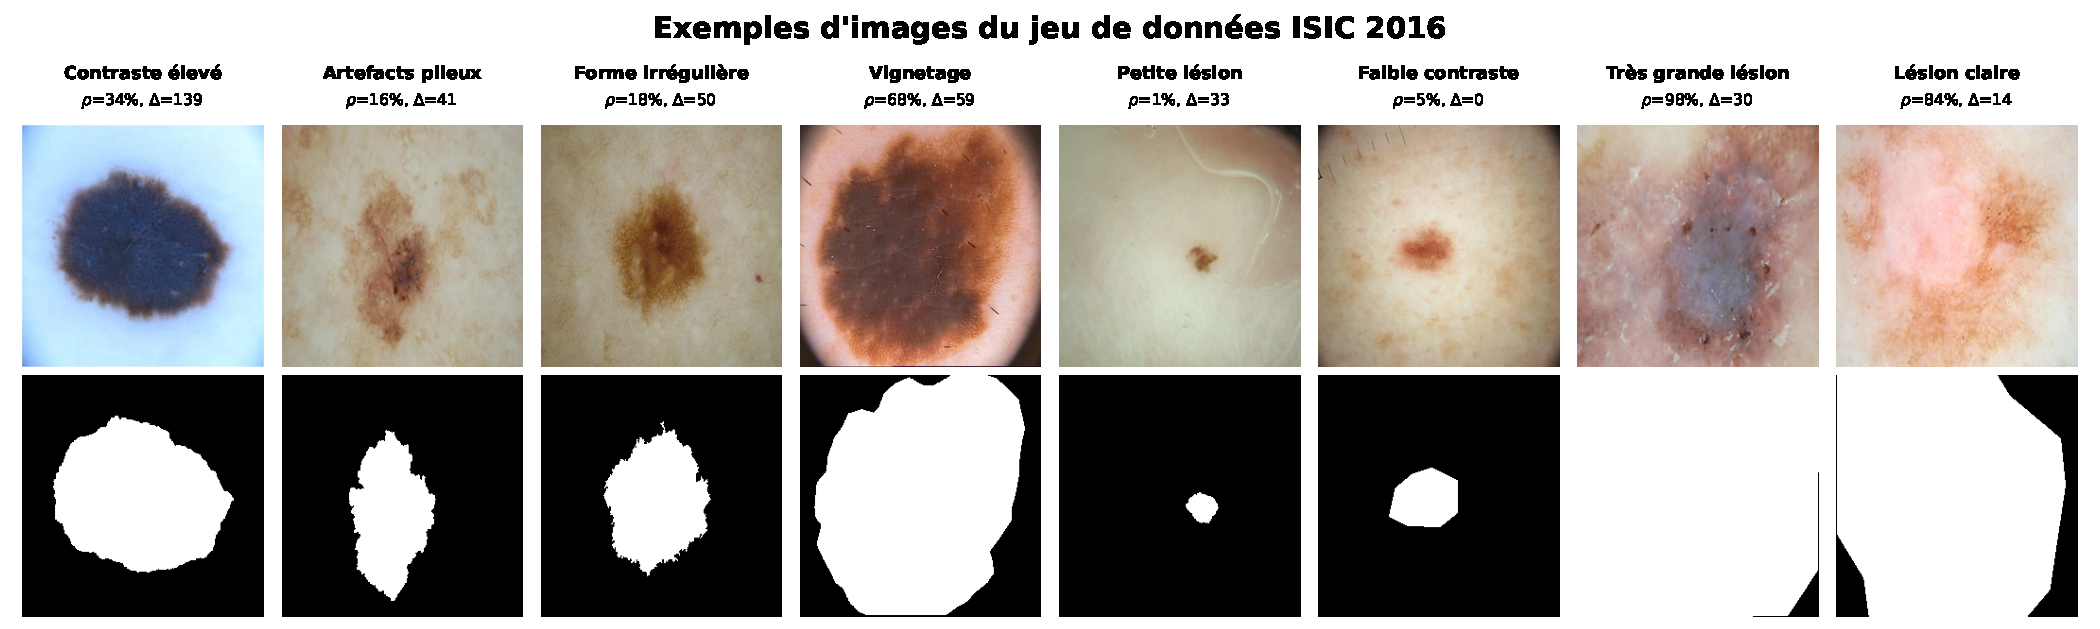
\includegraphics[width=\textwidth]{fig_dataset_examples.pdf}
\caption{Huit exemples représentatifs du jeu de données ISIC~2016 (ligne supérieure~: images dermoscopiques, ligne inférieure~: masques de référence). Le ratio lésion/image $\rho$ et le contraste $\Delta$ sont indiqués pour chaque cas. Les exemples illustrent les principaux défis~: contraste variable, artefacts pileux, vignettage, lésions de tailles extrêmes et lésions hypopigmentées.}
\label{fig:dataset_examples}
\end{figure}

\subsection{Prétraitement des masques}
\label{subsec:pretraitement}

Les masques de segmentation sont codés avec des valeurs discrètes $\{0, 255\}$~: la valeur $0$ correspond au fond (peau saine) et la valeur $255$ à la lésion. Un prétraitement de \textbf{binarisation} (conversion en $\{0, 1\}$) est appliqué systématiquement. Cette opération se justifie à trois titres~:
\begin{enumerate}[nosep]
    \item elle lève toute ambiguïté entre la notion d'\emph{intensité} (valeur de pixel) et celle d'\emph{étiquette} (classe sémantique)~;
    \item elle simplifie le calcul des métriques~: l'aire de la lésion correspond alors à $\sum_{i,j} M_{ij}$, où $M$ désigne le masque binarisé~;
    \item elle aligne le format des annotations avec les hypothèses des fonctions de perte standard en segmentation (Dice, IoU, entropie croisée binaire).
\end{enumerate}

\subsection{Analyse de la géométrie des images}
\label{subsec:geometrie}

L'analyse de la résolution des images révèle une \textbf{hétérogénéité marquée} des dimensions spatiales. Le tableau~\ref{tab:geometrie} synthétise les statistiques descriptives.

\begin{table}[H]
\centering
\caption{Statistiques descriptives de la géométrie des images ($n = 900$).}
\label{tab:geometrie}
\begin{tabular}{l r r r r r r}
\toprule
\textbf{Variable} & \textbf{Min} & \textbf{$Q_1$} & \textbf{Médiane} & \textbf{$Q_3$} & \textbf{Max} & \textbf{Moyenne $\pm$ écart-type} \\
\midrule
Largeur (px) & 576 & 1\,024 & 1\,024 & 2\,048 & 4\,288 & $1\,556 \pm 992$ \\
Hauteur (px) & 542 & 768 & 768 & 1\,536 & 2\,848 & $1\,133 \pm 656$ \\
Aire (px$^2$ $\times 10^3$) & 384 & 786 & 786 & 3\,146 & 12\,212 & $2\,409 \pm 3\,141$ \\
\bottomrule
\end{tabular}
\end{table}

La largeur varie d'un facteur~7,4 (de 576 à 4\,288 pixels) et la hauteur d'un facteur~5,3. Cette variabilité reflète l'utilisation de dispositifs d'acquisition différents au sein du jeu de données. Elle impose la mise en place d'une stratégie de \textbf{normalisation spatiale} en amont de tout modèle, typiquement via~:
\begin{itemize}[nosep]
    \item un \emph{redimensionnement} vers une taille fixe (par exemple $256 \times 256$ pixels), avec interpolation bilinéaire pour l'image et interpolation au plus proche voisin pour le masque~;
    \item un traitement par \emph{patches} (extraction de sous-images)~;
    \item une approche \emph{multi-échelle} combinant plusieurs résolutions.
\end{itemize}

\subsection{Distribution de la taille des lésions}
\label{subsec:taille}

La taille de la lésion est quantifiée par deux indicateurs~: l'aire absolue du masque binarisé (en pixels) et le \textbf{ratio lésion/image} $\rho$, défini comme la fraction de pixels de l'image appartenant à la lésion~:
\begin{equation}
    \rho = \frac{\sum_{i,j} M_{ij}}{H \times W}
    \label{eq:ratio}
\end{equation}
où $H$ et $W$ désignent respectivement la hauteur et la largeur de l'image. Le tableau~\ref{tab:taille_lesion} résume les statistiques observées.

\begin{table}[H]
\centering
\caption{Statistiques descriptives de la taille des lésions ($n = 900$).}
\label{tab:taille_lesion}
\begin{tabular}{l r r r r r}
\toprule
\textbf{Variable} & \textbf{Min} & \textbf{Médiane} & \textbf{Max} & \textbf{Moyenne} & \textbf{Écart-type} \\
\midrule
Aire du masque (px) & 9\,087 & 274\,133 & 5\,989\,020 & 431\,723 & 556\,843 \\
Ratio $\rho$ (\%) & 1,16 & 21,35 & 99,54 & 27,09 & 21,41 \\
\bottomrule
\end{tabular}
\end{table}

La répartition en classes de taille, présentée dans le tableau~\ref{tab:classes_taille}, confirme que la lésion occupe fréquemment une part substantielle de l'image ($\rho > 10\%$ dans 75,9\% des cas), tout en conservant une queue de distribution vers de petites lésions ($\rho \in [1\%, 5\%]$ dans 8,1\% des cas).

\begin{table}[H]
\centering
\caption{Répartition des lésions par classe de taille relative.}
\label{tab:classes_taille}
\begin{tabular}{l r r}
\toprule
\textbf{Classe de taille ($\rho$)} & \textbf{Effectif} & \textbf{Proportion} \\
\midrule
$< 1\%$ & 0 & 0,0\% \\
$1 - 5\%$ & 73 & 8,1\% \\
$5 - 10\%$ & 144 & 16,0\% \\
$> 10\%$ & 683 & 75,9\% \\
\bottomrule
\end{tabular}
\end{table}

La figure~\ref{fig:eda_distributions} présente la distribution de ces deux variables clés sous forme d'histogrammes, avec les seuils de catégorisation utilisés dans la suite de l'analyse.

\begin{figure}[H]
\centering
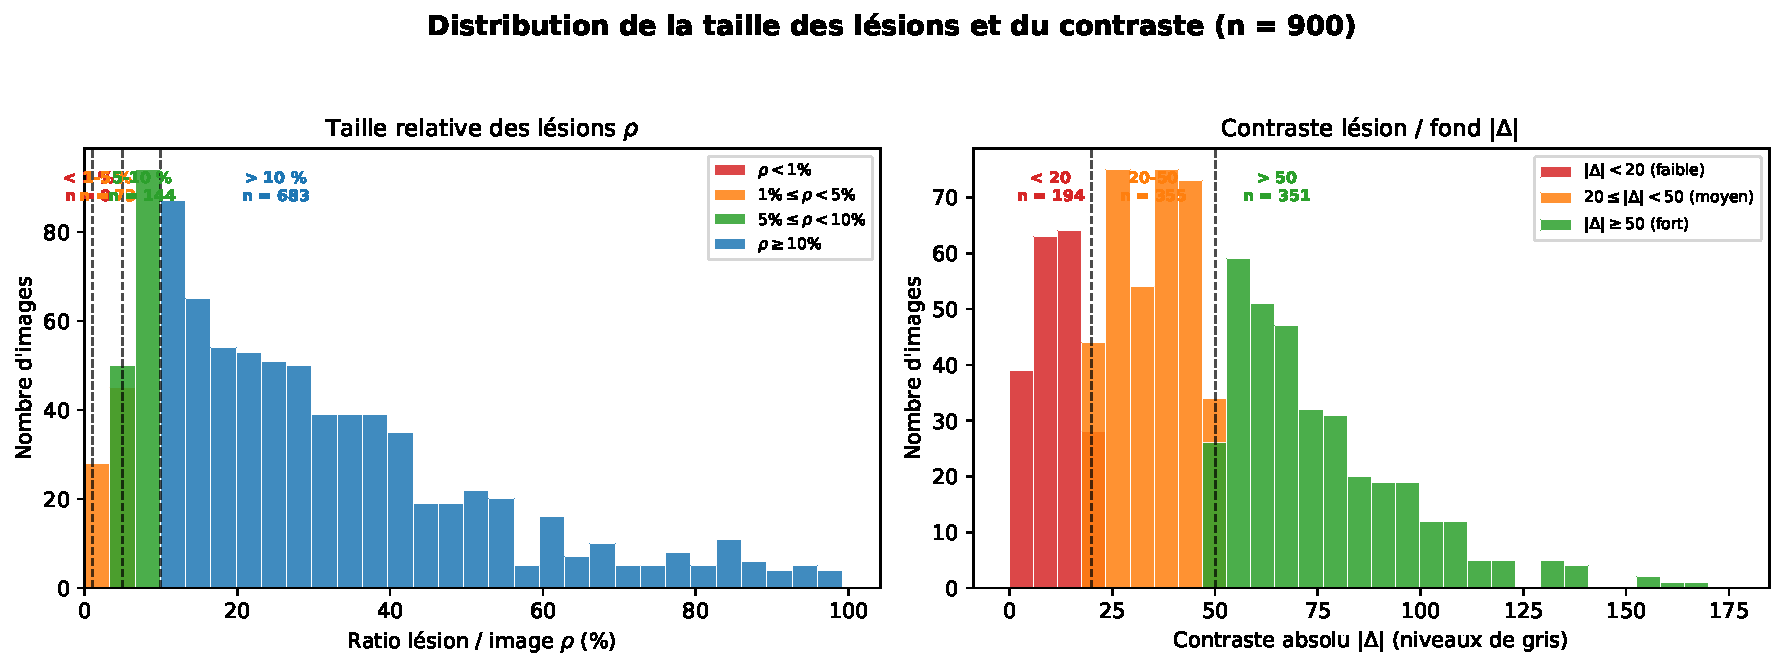
\includegraphics[width=\textwidth]{fig_eda_distributions.pdf}
\caption{Distribution de la taille relative des lésions $\rho$ (à gauche) et du contraste absolu lésion/fond $|\Delta|$ (à droite) sur les 900~images d'entraînement. Les lignes verticales pointillées indiquent les seuils de catégorisation utilisés dans l'analyse par sous-groupes.}
\label{fig:eda_distributions}
\end{figure}

Deux conséquences méthodologiques se dégagent de cette distribution~:

\paragraph{Déséquilibre de classes pour les petites lésions.} Les images à faible ratio $\rho$ induisent un fort déséquilibre entre pixels de fond et pixels de lésion. Ce déséquilibre favorise la sur-prédiction de la classe majoritaire (fond) par les modèles supervisés. Pour y remédier, des fonctions de perte adaptées à la classe rare --- Dice loss, IoU loss, entropie croisée binaire pondérée --- ainsi que des stratégies d'échantillonnage (recadrage centré sur la lésion, échantillonnage stratifié) peuvent être employées.

\paragraph{Ratios extrêmes.} L'existence de ratios atteignant $\rho \approx 99,5\%$ indique des images où la lésion recouvre la quasi-totalité du champ. Dans ces cas, la frontière lésion/fond est peu informative et les modèles deviennent plus dépendants de la texture et de l'illumination. Il est donc pertinent d'évaluer les performances par sous-groupes de ratio (petit, moyen, grand) plutôt que sur un score agrégé unique.

\subsection{Analyse topologique des masques}
\label{subsec:topologie}

L'analyse des composantes connexes de chaque masque binarisé, réalisée par étiquetage (\emph{connected component labeling}) en 4-connexité, révèle que la grande majorité des images ne contient qu'une seule composante connexe. Seules \textbf{6 images} (0,7\% du corpus) présentent des composantes multiples. L'examen visuel de ces cas montre qu'il s'agit d'artefacts d'annotation (petites régions isolées de quelques pixels) plutôt que de véritables lésions distinctes.

Cette quasi-unicité topologique a deux implications~:
\begin{itemize}[nosep]
    \item Un \textbf{post-traitement simple} --- consistant à ne conserver que la plus grande composante connexe du masque prédit et à éliminer les petites composantes par seuil d'aire --- suffit à nettoyer les prédictions bruitées tout en respectant l'hypothèse d'une lésion principale par image.
    \item L'hypothèse d'unicité de la lésion rend viable une approche de \textbf{segmentation non supervisée par $K$-means} avec $K = 2$ (lésion vs. fond), en augmentant éventuellement l'espace de caractéristiques des coordonnées spatiales $(x, y)$ pour favoriser la compacité des régions.
\end{itemize}

\subsection{Localisation spatiale des lésions}
\label{subsec:centroide}

La position de chaque lésion est caractérisée par le centroïde (barycentre géométrique) de la plus grande composante connexe, exprimé en coordonnées normalisées dans $[0, 1]$ (où $0$ correspond au bord supérieur/gauche et $1$ au bord inférieur/droit). Le tableau~\ref{tab:centroide} présente les statistiques de localisation.

\begin{table}[H]
\centering
\caption{Statistiques de localisation des centroïdes ($n = 900$).}
\label{tab:centroide}
\begin{tabular}{l r r r r r}
\toprule
\textbf{Variable} & \textbf{Min} & \textbf{Médiane} & \textbf{Max} & \textbf{Moyenne} & \textbf{Écart-type} \\
\midrule
$x$ normalisé & 0,195 & 0,490 & 0,807 & 0,484 & 0,061 \\
$y$ normalisé & 0,237 & 0,501 & 0,690 & 0,499 & 0,056 \\
Distance au centre (px) & 1,98 & 52,05 & 1\,239 & 109,50 & 162,66 \\
\bottomrule
\end{tabular}
\end{table}

Les centroïdes sont en moyenne proches du centre de l'image ($\bar{x} = 0{,}484$, $\bar{y} = 0{,}499$), ce qui reflète le protocole d'acquisition dermoscopique standard, où le praticien centre le dermatoscope sur la lésion. Toutefois, la distance maximale au centre (1\,239~pixels) témoigne de l'existence de lésions significativement excentrées.

Ce biais de centrage justifie le recours à des \textbf{augmentations géométriques} (retournements horizontaux et verticaux) lors de l'entraînement des modèles supervisés afin de réduire leur sensibilité à la position de la lésion dans l'image.

\subsection{Analyse photométrique et contraste lésion/fond}
\label{subsec:photometrie}

L'intensité moyenne de chaque image est calculée par canal (R, G, B) puis convertie en niveaux de gris selon la formule de luminance ITU-R BT.601~:
\begin{equation}
    I_{\text{gris}} = 0{,}299 \cdot R + 0{,}587 \cdot G + 0{,}114 \cdot B
    \label{eq:gris}
\end{equation}

Le tableau~\ref{tab:intensite} présente les statistiques d'intensité par canal et en niveaux de gris.

\begin{table}[H]
\centering
\caption{Intensité moyenne par image, par canal et en niveaux de gris ($n = 900$, échelle $[0, 255]$).}
\label{tab:intensite}
\begin{tabular}{l r r r r}
\toprule
\textbf{Canal} & \textbf{Min} & \textbf{Médiane} & \textbf{Max} & \textbf{Moyenne $\pm$ écart-type} \\
\midrule
Rouge (R) & 77,4 & 183,0 & 246,7 & $184{,}6 \pm 28{,}4$ \\
Vert (G) & 63,6 & 154,1 & 232,4 & $157{,}8 \pm 25{,}4$ \\
Bleu (B) & 52,7 & 142,8 & 230,8 & $144{,}6 \pm 26{,}9$ \\
Gris & 75,6 & 162,0 & 233,2 & $164{,}3 \pm 24{,}6$ \\
\bottomrule
\end{tabular}
\end{table}

Le contraste lésion/fond est analysé en comparant l'intensité moyenne en niveaux de gris des pixels appartenant à la lésion ($\bar{I}_{\text{lésion}}$) à celle des pixels du fond ($\bar{I}_{\text{fond}}$). Le tableau~\ref{tab:contraste} résume ces résultats.

\begin{table}[H]
\centering
\caption{Contraste lésion/fond en niveaux de gris ($n = 900$).}
\label{tab:contraste}
\begin{tabular}{l r r r r}
\toprule
\textbf{Variable} & \textbf{Min} & \textbf{Médiane} & \textbf{Max} & \textbf{Moyenne} \\
\midrule
$\bar{I}_{\text{lésion}}$ & 47,9 & 130,9 & 215,9 & 132,2 \\
$\bar{I}_{\text{fond}}$ & 38,5 & 173,7 & 248,4 & 176,3 \\
$\Delta = \bar{I}_{\text{lésion}} - \bar{I}_{\text{fond}}$ & $-167{,}7$ & $-41{,}0$ & $+110{,}0$ & $-44{,}0$ \\
$|\Delta|$ & 0,01 & 41,7 & 167,7 & 45,7 \\
\bottomrule
\end{tabular}
\end{table}

Le contraste moyen est négatif ($\bar{\Delta} = -44{,}0$), indiquant que la lésion est en moyenne \textbf{plus sombre} que la peau environnante. Ce résultat, cohérent avec la physique de la dermoscopie (absorption accrue de la lumière par la mélanine), se vérifie dans \textbf{96,1\%} des images. Les 3,9\% restants correspondent à des cas de contraste inversé, attribuables à des variations d'éclairage, des types de lésions hypopigmentées, ou des artefacts optiques (reflets spéculaires, bulles).

Pour la modélisation, ce résultat appelle trois recommandations~:
\begin{enumerate}[nosep]
    \item Le contraste d'intensité est un indice discriminant mais insuffisant à lui seul~: le modèle doit également exploiter les caractéristiques de \textbf{texture} et de \textbf{contexte spatial}.
    \item Une \textbf{normalisation par image} (standardisation des canaux, égalisation d'histogramme) et des \textbf{augmentations photométriques} (jitter de luminosité, contraste, saturation) sont recommandées pour renforcer la robustesse.
    \item Les cas de contraste faible ($|\Delta| \approx 0$) représentent les instances les plus difficiles et méritent une \textbf{analyse d'erreurs ciblée} lors de l'évaluation des modèles.
\end{enumerate}

\subsection{Synthèse de l'analyse exploratoire}

En synthèse, le jeu de données ISIC~2016 constitue un corpus cohérent et adapté à la segmentation supervisée de lésions cutanées, malgré une variabilité significative selon plusieurs axes~: résolution des images, taille relative de la lésion, qualité topologique des masques, position des lésions, et contraste photométrique. Le tableau~\ref{tab:synthese} récapitule les caractéristiques saillantes et leurs implications méthodologiques.

\begin{table}[H]
\centering
\caption{Synthèse des caractéristiques du jeu de données et implications pour la modélisation.}
\label{tab:synthese}
\small
\begin{tabular}{p{4cm} p{4.5cm} p{5cm}}
\toprule
\textbf{Caractéristique} & \textbf{Observation} & \textbf{Implication méthodologique} \\
\midrule
Résolution & Forte hétérogénéité (576--4\,288~px) & Redimensionnement à taille fixe ou traitement par patches \\
\addlinespace
Taille des lésions & $\rho \in [1{,}2\%, 99{,}5\%]$, 75,9\% $> 10\%$ & Fonctions de perte adaptées (Dice, IoU), évaluation par sous-groupes \\
\addlinespace
Topologie des masques & 99,3\% mono-composante & Post-traitement par composante maximale \\
\addlinespace
Localisation & Tendance au centrage, excentrements possibles & Augmentations géométriques \\
\addlinespace
Contraste & Lésion plus sombre dans 96,1\% des cas & Normalisation par image, augmentations photométriques \\
\bottomrule
\end{tabular}
\end{table}


% ══════════════════════════════════════════════
% 4. MÉTHODOLOGIE
% ══════════════════════════════════════════════
\section{Méthodologie}
\label{sec:methodologie}

\subsection{Formalisation du problème de segmentation}

Le problème de segmentation binaire peut être formalisé comme suit. Soit $\mathbf{X} \in \R^{H \times W \times C}$ une image d'entrée de hauteur $H$, de largeur $W$ et de $C$ canaux (typiquement $C = 3$ pour une image RGB). L'objectif est d'apprendre une fonction $f_\theta : \R^{H \times W \times C} \to \{0, 1\}^{H \times W}$ qui associe à chaque pixel $(i, j)$ une étiquette binaire~:
\begin{equation}
    f_\theta(\mathbf{X})_{ij} =
    \begin{cases}
        1 & \text{si le pixel $(i, j)$ appartient à la lésion,} \\
        0 & \text{sinon (fond).}
    \end{cases}
\end{equation}

Dans le cadre supervisé, les paramètres $\theta$ sont estimés en minimisant une fonction de perte $\mathcal{L}$ sur un ensemble d'entraînement $\{(\mathbf{X}^{(k)}, \mathbf{Y}^{(k)})\}_{k=1}^{N}$, où $\mathbf{Y}^{(k)}$ désigne le masque de référence~:
\begin{equation}
    \hat{\theta} = \argmin_\theta \frac{1}{N} \sum_{k=1}^{N} \mathcal{L}\big(f_\theta(\mathbf{X}^{(k)}),\, \mathbf{Y}^{(k)}\big)
    \label{eq:optim}
\end{equation}

\subsection{Segmentation par $K$-means}
\label{subsec:kmeans}

\subsubsection{Principe de l'algorithme}

L'algorithme des $K$-means \citep{macqueen1967kmeans} est une méthode de partitionnement non supervisé qui vise à répartir un ensemble de $n$ observations $\{\mathbf{z}_1, \ldots, \mathbf{z}_n\} \subset \R^d$ en $K$ groupes $\{C_1, \ldots, C_K\}$ en minimisant l'inertie intra-classes~:
\begin{equation}
    \min_{C_1, \ldots, C_K} \sum_{k=1}^{K} \sum_{\mathbf{z}_i \in C_k} \|\mathbf{z}_i - \boldsymbol{\mu}_k\|^2
    \label{eq:kmeans}
\end{equation}
où $\boldsymbol{\mu}_k = \frac{1}{|C_k|} \sum_{\mathbf{z}_i \in C_k} \mathbf{z}_i$ est le centroïde du cluster $C_k$.

L'algorithme procède par itérations alternées~: (i) \emph{assignation} de chaque observation au cluster dont le centroïde est le plus proche, et (ii) \emph{mise à jour} des centroïdes. La convergence vers un minimum local de l'inertie est garantie, mais le résultat dépend de l'initialisation (typiquement résolue par la stratégie $K$-means++ \citep{arthur2007kmeans++}).

\subsubsection{Application à la segmentation de lésions cutanées}

Dans le contexte de la segmentation, chaque pixel $(i, j)$ de l'image est représenté par un vecteur de caractéristiques $\mathbf{z}_{ij} \in \R^d$. L'algorithme des $K$-means est appliqué à l'ensemble des pixels pour produire une partition en $K$ clusters, dont l'un est assigné à la classe \og lésion \fg{} et les autres au \og fond \fg{}. Un post-traitement systématique est appliqué~: seule la \textbf{plus grande composante connexe} du cluster assigné à la lésion est conservée, afin d'éliminer les régions parasites (artefacts de poils, ombres locales), conformément à l'hypothèse d'unicité topologique établie en section~\ref{subsec:topologie}.

\subsubsection{Espaces colorimétriques}
\label{subsubsec:espaces_couleur}

L'espace de caractéristiques dans lequel opère le $K$-means conditionne fortement la qualité de la partition obtenue. Quatre variantes ont été évaluées, chacune mettant en jeu un compromis différent entre information colorimétrique, perceptuelle et spatiale~:
\begin{enumerate}[nosep]
    \item \textbf{RGB}~: $\mathbf{z}_{ij} = (R_{ij}, G_{ij}, B_{ij})^\top \in \R^3$. Espace natif de l'image, simple mais sensible aux variations d'illumination.
    \item \textbf{RGB + coordonnées spatiales}~: $\mathbf{z}_{ij} = (R_{ij}, G_{ij}, B_{ij}, \alpha \cdot \tilde{x}_{ij}, \alpha \cdot \tilde{y}_{ij})^\top \in \R^5$, avec $\tilde{x}_{ij}, \tilde{y}_{ij} \in [0, 1]$ les coordonnées normalisées et $\alpha = 50$ un facteur de pondération. L'ajout des coordonnées spatiales favorise la compacité géographique des clusters, au prix d'un biais de position.
    \item \textbf{CIE~LAB}~: $\mathbf{z}_{ij} = (L^*_{ij}, a^*_{ij}, b^*_{ij})^\top \in \R^3$. Cet espace, conçu pour être perceptuellement uniforme, découple la luminance ($L^*$) de la chrominance ($a^*$, $b^*$), ce qui le rend moins sensible aux variations d'éclairage.
    \item \textbf{HSV}~: $\mathbf{z}_{ij} = (H_{ij}, S_{ij}, V_{ij})^\top \in \R^3$. La séparation entre teinte ($H$), saturation ($S$) et valeur ($V$) offre une représentation intuitive, mais la circularité de la teinte peut poser des difficultés au $K$-means (discontinuité à $H = 0° \equiv 360°$).
\end{enumerate}

\subsubsection{Règle d'assignation du cluster lésion}
\label{subsubsec:assignation}

Après convergence du $K$-means, il reste à déterminer lequel des $K$ clusters correspond à la lésion. Deux heuristiques ont été évaluées~:

\paragraph{Heuristique de luminosité (\og sombre \fg{}).} Le cluster dont l'intensité moyenne en niveaux de gris (équation~\ref{eq:gris}) est la plus faible est assigné à la lésion. Cette règle est motivée par l'observation photométrique de la section~\ref{subsec:photometrie}~: dans 96{,}1\% des images, la lésion est plus sombre que le fond.

\paragraph{Heuristique de centralité.} Le cluster le plus représenté dans la zone centrale de l'image (quart central, soit le rectangle $[H/4,\, 3H/4] \times [W/4,\, 3W/4]$) est assigné à la lésion. Cette règle exploite le biais de centrage identifié en section~\ref{subsec:centroide} ($\bar{x} \approx 0{,}49$, $\bar{y} \approx 0{,}50$) et s'avère a priori pertinente lorsque $K > 2$, car elle ne repose pas sur l'hypothèse que la lésion est le cluster \emph{le plus} sombre parmi $K$.

\subsubsection{Estimation du nombre optimal de clusters}
\label{subsubsec:estimation_k}

L'approche la plus simple consiste à fixer $K = 2$ (lésion vs.\ fond). Cependant, les images dermoscopiques contiennent fréquemment des éléments parasites (poils, bulles d'air, reflets, bordures de dermatoscope) susceptibles de former des classes colorimétriques distinctes. Afin de déterminer si un $K$ adaptatif, estimé image par image, pourrait améliorer la segmentation, trois méthodes d'estimation ont été mises en \oe uvre pour $K \in \{2, 3, 4, 5, 6\}$~:

\begin{itemize}[nosep]
    \item \textbf{Méthode du coude (\emph{Elbow})}~: on identifie le \og coude \fg{} de la courbe d'inertie intra-classe $W_K$ vs.\ $K$, c'est-à-dire le point au-delà duquel le gain marginal devient négligeable.
    \item \textbf{Score de silhouette}~: pour chaque point, on mesure le rapport entre la cohésion intra-cluster et la séparation inter-cluster. Le $K$ optimal maximise le score moyen $\bar{s}(K) \in [-1, 1]$.
    \item \textbf{BIC via mélange gaussien (GMM)}~: un modèle de mélange de $K$ gaussiennes est ajusté par l'algorithme EM. Le \emph{Bayesian Information Criterion}, qui pénalise la vraisemblance par la complexité du modèle, est minimisé.
\end{itemize}

Pour des raisons de complexité calculatoire, les estimations sont réalisées sur un \textbf{sous-échantillon de 10\,000~pixels} par image.

\subsubsection{Protocole expérimental}
\label{subsubsec:protocole_kmeans}

L'évaluation de la segmentation par $K$-means s'organise en deux volets~:

\paragraph{Évaluation des espaces colorimétriques.} Les quatre variantes (RGB, RGB+spatial, LAB, HSV) sont évaluées avec $K = 2$ et l'heuristique de luminosité sur l'\textbf{intégralité des 900~images}. Les métriques reportées sont le DSC, l'IoU, la \emph{pixel accuracy}, la précision et le rappel. Les performances sont analysées globalement puis par sous-groupes de difficulté~: taille de la lésion ($\rho < 5\%$, $5\% \leq \rho < 10\%$, $\rho \geq 10\%$), contraste ($|\Delta| < 20$, $20 \leq |\Delta| < 50$, $|\Delta| \geq 50$) et présence de vignettage.

\paragraph{Étude d'ablation $K \times$ assignation.} Un sous-ensemble stratifié de \textbf{225~images} (25\% du corpus) est constitué par \texttt{StratifiedShuffleSplit} sur les classes de taille $\rho$, garantissant une distribution homogène des sous-groupes. Sur ce sous-ensemble, quatre configurations sont comparées dans une grille $2 \times 2$~:
\begin{center}
\small
\begin{tabular}{l c c}
\toprule
 & \textbf{Sombre} & \textbf{Centralité} \\
\midrule
$K = 2$ fixe & Baseline & Effet assignation \\
$K$ adaptatif (silhouette) & Effet de $K$ & Effet combiné \\
\bottomrule
\end{tabular}
\end{center}
Cette grille permet d'isoler l'effet marginal de chaque facteur~: la règle d'assignation (à $K$ fixé) et le choix de $K$ (à règle fixée).

\subsubsection{Limites identifiées~: l'effet de loupe}
\label{subsubsec:loupe}

Un phénomène récurrent, que nous désignons par \textbf{effet de loupe} (ou \emph{vignettage}), est observé sur les images acquises avec un dermatoscope à contact. Ces images présentent une zone circulaire correspondant au champ de vision de l'instrument, entourée d'une bordure sombre hors du champ optique. Or, cette bordure est colorimétriquement plus proche de la lésion (elle aussi plus sombre que la peau) que du fond clair. En conséquence, l'algorithme $K$-means attribue les pixels de la bordure au même cluster que la lésion, produisant un masque erroné. La détection de ce phénomène est réalisée par une heuristique simple~: une image est classée comme présentant un vignettage si l'intensité moyenne des pixels situés dans une bande de 5\% de la largeur le long des bords est inférieure à un seuil de 40 (sur $[0, 255]$).

\subsection{Segmentation par CNN sur patches}
\label{subsec:cnn_patch_methodo}

La seconde approche constitue une étape intermédiaire entre le $K$-means et le U-Net, inspirée des travaux de \citet{ciresan2012deep} sur la segmentation de membranes neuronales par classification de patches. Plutôt que de traiter l'image entière, on extrait pour chaque pixel un \textbf{patch carré} centré sur ce pixel, puis un réseau convolutif (\emph{CNN}) classifie ce patch comme « lésion » ou « fond ». Cette approche introduit deux ingrédients absents du $K$-means~: (i)~des \textbf{convolutions apprises}, qui capturent des motifs locaux (texture, gradient) au-delà de la seule information colorimétrique~; (ii)~une \textbf{supervision}, qui permet d'adapter les représentations à la tâche.

\subsubsection{Extraction des patches}

Soit $I \in [0, 1]^{H \times W \times 3}$ une image et $M \in \{0, 1\}^{H \times W}$ le masque binaire associé ($H = W = 256$). Pour chaque pixel $(i, j)$ situé à distance suffisante des bords ($i \in [\frac{P}{2},\, H - \frac{P}{2}]$, idem pour $j$), on définit le patch centré~:
\begin{equation}
    \mathcal{P}_{ij} = I\!\left[i - \tfrac{P}{2}\,:\,i + \tfrac{P}{2},\; j - \tfrac{P}{2}\,:\,j + \tfrac{P}{2},\; :\right] \in [0, 1]^{P \times P \times 3}
    \label{eq:patch}
\end{equation}
Le label associé est $y_{ij} = M_{ij} \in \{0, 1\}$. L'ensemble des pixels valides est partitionné en deux classes~: $\Omega_1 = \{(i,j) : M_{ij} = 1\}$ (lésion) et $\Omega_0 = \{(i,j) : M_{ij} = 0\}$ (fond). Pour chaque image, on échantillonne aléatoirement $n = 100$ pixels de chaque classe~:
\begin{equation}
    S_k \subset \Omega_k, \quad |S_k| = \min(n, |\Omega_k|), \quad k \in \{0, 1\}
    \label{eq:sampling}
\end{equation}
Cet \textbf{échantillonnage équilibré} (50/50) est essentiel~: le fond domine la plupart des images (ratio médian $\rho \approx 21\%$, section~\ref{subsec:taille}), ce qui biaiserait l'entraînement vers la classe majoritaire sans cette correction. Au total, l'extraction produit environ $126\,000$ patches d'entraînement ($630 \times 2 \times 100$) et $36\,000$ patches de validation ($180 \times 2 \times 100$), en utilisant le même split stratifié que le U-Net (section~\ref{subsec:protocole_entrainement}, seed $= 42$).

\subsubsection{Architecture du CNN}
\label{subsubsec:archi_cnn_patch}

Le réseau est volontairement simple --- 3 blocs convolutifs suivis de couches denses --- afin d'isoler l'apport des convolutions apprises sans bénéficier de la structure encodeur-décodeur du U-Net~:
\begin{equation}
    f_\theta : \R^{P \times P \times 3} \to [0, 1], \quad \mathcal{P}_{ij} \mapsto \hat{p}_{ij} = \sigma\!\big(g_\theta(\mathcal{P}_{ij})\big)
    \label{eq:cnn_patch}
\end{equation}
où $\sigma$ désigne la fonction sigmoïde et $g_\theta$ le réseau composé de~:
\begin{itemize}[nosep]
    \item \textbf{Bloc 1}~: $\text{Conv2D}(32, 3 \times 3) \times 2 + \text{MaxPool}(2 \times 2)$
    \item \textbf{Bloc 2}~: $\text{Conv2D}(64, 3 \times 3) \times 2 + \text{MaxPool}(2 \times 2)$
    \item \textbf{Bloc 3}~: $\text{Conv2D}(128, 3 \times 3) + \text{MaxPool}(2 \times 2)$
    \item \textbf{Classification}~: $\text{GlobalAveragePooling2D} \to \text{Dense}(64, \text{ReLU}) \to \text{Dropout}(0{,}5) \to \text{Dense}(1, \sigma)$
\end{itemize}
Toutes les convolutions utilisent le padding \texttt{same}, l'activation ReLU et l'initialisation He normal. Le $\text{GlobalAveragePooling2D}$ rend le modèle agnostique à la taille exacte du patch, ce qui permet de comparer directement $P \in \{32, 48, 64\}$ avec la \textbf{même architecture} (147\,745 paramètres dans chaque cas).

\paragraph{Fonction de perte.} La fonction de perte retenue est l'\textbf{entropie croisée binaire} (BCE, équation~\ref{eq:bce}). Contrairement au U-Net, où la Dice loss est nécessaire pour compenser le déséquilibre pixel-level (le fond domine chaque masque), le CNN patch opère sur un dataset de patches \textbf{déjà équilibré} par construction (50\% lésion, 50\% fond). La BCE est donc le choix canonique pour ce problème de classification binaire.

\subsubsection{Inférence par fenêtre glissante}
\label{subsubsec:inference_patch}

Le CNN classifie des patches individuels ; la reconstruction d'un masque complet nécessite une procédure d'inférence spécifique. On parcourt l'image avec une \textbf{fenêtre glissante} de pas (\emph{stride}) $s$. Pour chaque position valide $(i, j)$, le CNN prédit la probabilité $\hat{p}_{ij} = f_\theta(\mathcal{P}_{ij})$. On obtient une grille de probabilités à résolution réduite~:
\begin{equation}
    G \in [0, 1]^{N_y \times N_x}, \quad N_y = \left\lfloor\frac{H - P}{s}\right\rfloor + 1, \quad N_x = \left\lfloor\frac{W - P}{s}\right\rfloor + 1
    \label{eq:grid}
\end{equation}
Pour $P = 32$ et $s = 8$, on obtient $N_y = N_x = 28$, soit $784$ évaluations du CNN par image. Cette grille est ensuite redimensionnée à la résolution originale par \textbf{interpolation bilinéaire}~: $\hat{M} = \text{Resize}(G, H \times W)$. Le masque binaire final est obtenu par binarisation au seuil $\tau = 0{,}5$, suivie du même \textbf{post-traitement} que pour le $K$-means~: conservation de la plus grande composante connexe (section~\ref{subsec:kmeans}).

\paragraph{Coût d'inférence.} Cette procédure nécessite $N_y \times N_x$ évaluations du CNN par image, contre \textbf{un seul passage} (\emph{forward pass}) pour le U-Net. Ce coût, intrinsèque à l'approche par patches, constitue une limitation importante en pratique clinique.

\subsubsection{Protocole d'entraînement et d'ablation}
\label{subsubsec:protocole_cnn_patch}

Le protocole d'entraînement est le suivant~: optimiseur \textbf{Adam} ($\eta = 10^{-4}$), 30 epochs maximum avec \textbf{early stopping} (patience $= 5$, restauration des meilleurs poids selon la \texttt{val\_loss}), taille de mini-batch $= 64$, augmentation par retournements horizontaux et verticaux aléatoires.

La taille du patch $P$ contrôle le \textbf{champ réceptif} du CNN~: un patch plus grand fournit davantage de contexte mais risque d'inclure du fond non informatif. Afin de quantifier cet effet, on réalise une étude d'ablation sur $P \in \{32, 48, 64\}$ en entraînant un modèle indépendant pour chaque configuration, tous les autres hyperparamètres restant fixés. Le stride d'inférence est fixé à $s = 8$ pour $P = 32$ et $P = 48$, et augmenté à $s = 10$ pour $P = 64$ afin de maintenir un nombre de positions d'évaluation comparable ($\sim 625$--$784$) et un temps d'inférence raisonnable.

\subsection{Architecture U-Net}
\label{subsec:unet_methodo}

La troisième approche repose sur l'architecture U-Net \citep{ronneberger2015unet}, décrite en section~\ref{subsec:unet}. La figure~\ref{fig:unet_archi} illustre la configuration de base retenue. L'implémentation est \textbf{entièrement paramétrable}, ce qui permet de faire varier systématiquement chaque composant lors de l'étude d'ablation (section~\ref{subsec:ablation_protocole}). Les hyperparamètres architecturaux configurables sont~:
\begin{itemize}[nosep]
    \item \texttt{base\_filters}~: nombre de filtres dans le premier bloc convolutif (32, 64 ou 128), doublé à chaque niveau de profondeur~;
    \item \texttt{depth}~: nombre de niveaux de l'encodeur (3, 4 ou 5)~;
    \item \texttt{use\_skip}~: activation ou désactivation des \emph{skip connections}~;
    \item \texttt{dropout}~: taux de \emph{dropout} appliqué après chaque bloc convolutif (0, 0{,}2 ou 0{,}5)~;
    \item \texttt{upsample}~: méthode de sur-échantillonnage dans le décodeur (interpolation bilinéaire ou convolution transposée)~;
    \item \texttt{pooling}~: type de sous-échantillonnage dans l'encodeur (\emph{max-pooling} ou \emph{average pooling})~;
    \item \texttt{batchnorm}~: activation ou désactivation de la normalisation par lot \citep{ioffe2015batchnorm}.
\end{itemize}

Dans la configuration de base (\texttt{base\_filters=64}, \texttt{depth=4}, \texttt{use\_skip=True}, \texttt{batchnorm=True}, \texttt{pooling=max}, \texttt{upsample=bilinear}, \texttt{dropout=0}), le réseau totalise \textbf{31,4 millions de paramètres}.

\begin{figure}[H]
\centering
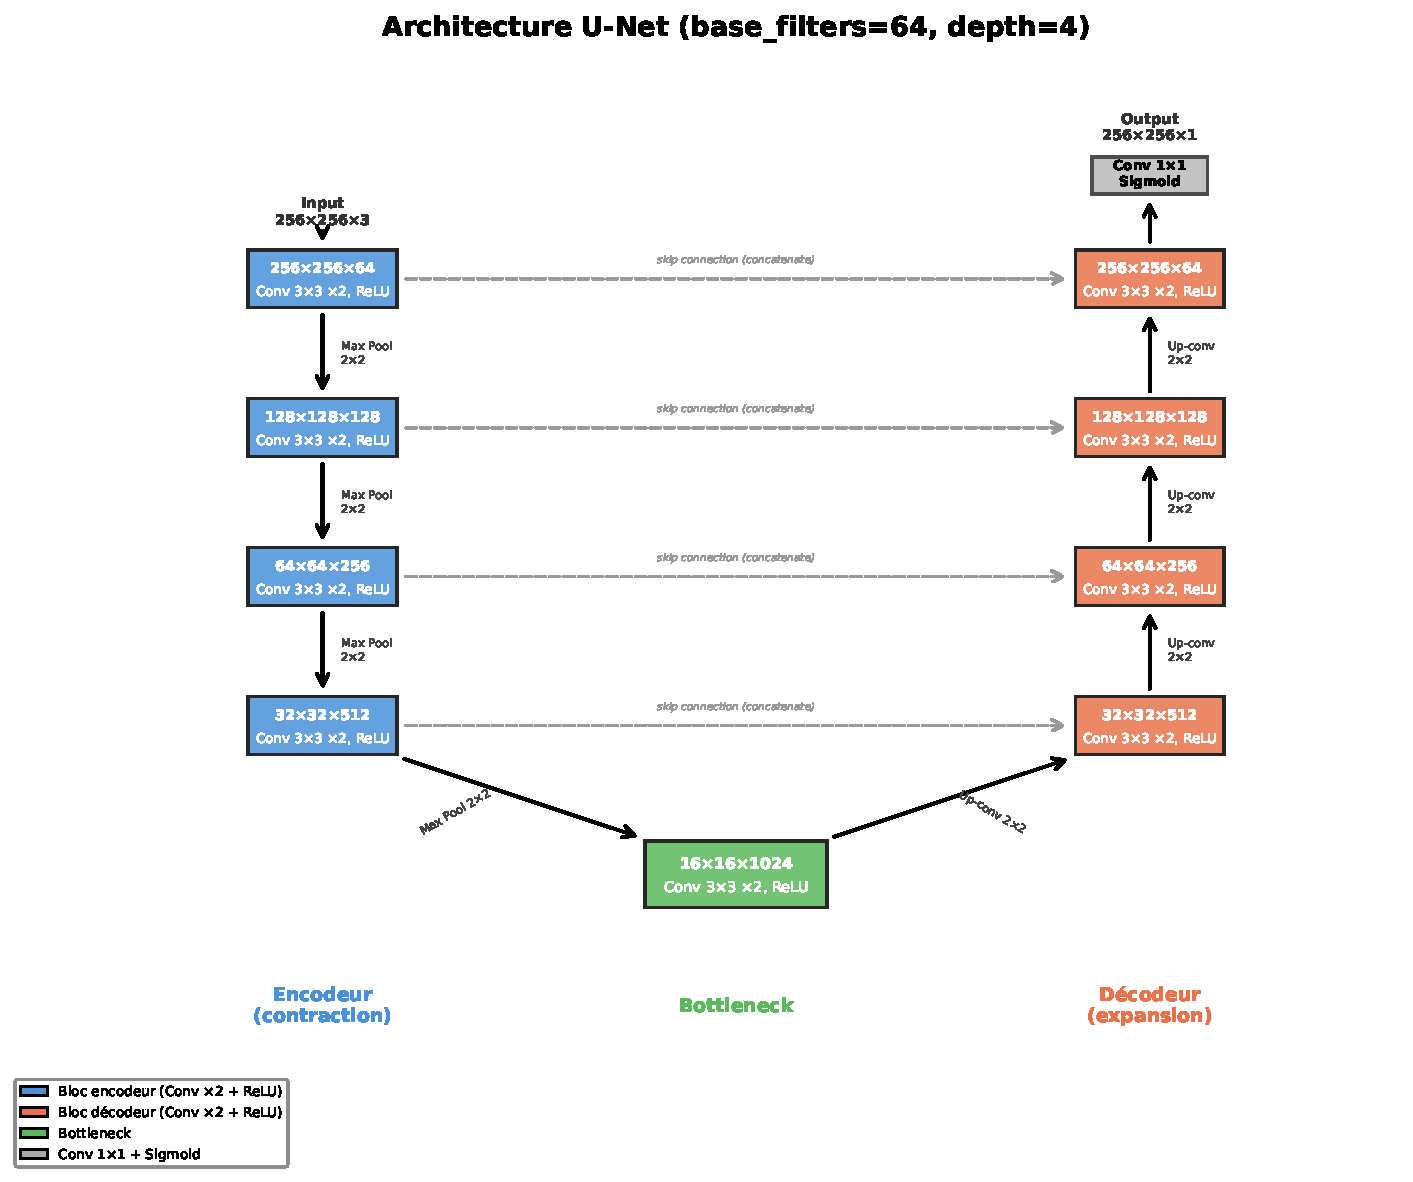
\includegraphics[width=0.85\textwidth]{fig_unet_architecture.pdf}
\caption{Architecture U-Net dans sa configuration de base (\texttt{base\_filters=64}, \texttt{depth=4}). L'encodeur (bleu) réduit progressivement la résolution spatiale tout en augmentant le nombre de filtres. Le bottleneck (vert) opère à la résolution la plus basse ($16 \times 16$). Le décodeur (orange) reconstruit la résolution originale. Les connexions résiduelles (flèches pointillées) concatènent les cartes de caractéristiques de l'encodeur au décodeur à chaque niveau.}
\label{fig:unet_archi}
\end{figure}

\paragraph{Fonctions de perte.} Quatre fonctions de perte ont été évaluées~:
\begin{enumerate}[nosep]
    \item \textbf{Entropie croisée binaire (BCE)}~:
    \begin{equation}
        \mathcal{L}_{\text{BCE}} = -\frac{1}{HW}\sum_{i,j} \Big[Y_{ij} \log \hat{Y}_{ij} + (1 - Y_{ij}) \log(1 - \hat{Y}_{ij})\Big]
        \label{eq:bce}
    \end{equation}
    \item \textbf{Dice loss}~: $\mathcal{L}_{\text{Dice}} = 1 - \text{DSC}(Y, \hat{Y})$, directement dérivée du coefficient de Dice (équation~\ref{eq:dice}).
    \item \textbf{IoU loss}~: $\mathcal{L}_{\text{IoU}} = 1 - \text{IoU}(Y, \hat{Y})$, dérivée de l'indice de Jaccard (équation~\ref{eq:iou}).
    \item \textbf{BCE + Dice}~: combinaison linéaire $\mathcal{L} = \mathcal{L}_{\text{Dice}} + \lambda\, \mathcal{L}_{\text{BCE}}$, avec $\lambda = 1$.
\end{enumerate}

Une variante avec \textbf{pondération aux frontières} (\emph{boundary-weighted loss}) a également été testée. Le masque de poids est construit par dilatation morphologique du contour de la lésion (noyau $3 \times 3$, 3 itérations), attribuant un poids $w \in \{5, 10\}$ aux pixels situés dans cette bande frontière et un poids unitaire ailleurs. L'objectif est d'encourager une segmentation plus précise des bords, où les erreurs ont le plus d'impact clinique.

\subsection{Protocole d'entraînement}
\label{subsec:protocole_entrainement}

L'ensemble des expériences a été réalisé sur un GPU \textbf{NVIDIA Tesla T4} (16~Go VRAM). Les 900 images d'entraînement sont partitionnées par un \textbf{split stratifié} (\texttt{StratifiedShuffleSplit}) selon la taille relative de la lésion $\rho$ (section~\ref{subsec:taille}), garantissant une distribution homogène des classes de taille~:
\begin{itemize}[nosep]
    \item \textbf{Entraînement}~: 80\% (720 images)~;
    \item \textbf{Validation}~: 20\% (180 images).
\end{itemize}
L'évaluation finale est réalisée sur le \textbf{jeu de test officiel ISBI~2016} (379 images), totalement indépendant et jamais vu pendant l'entraînement ni la sélection de modèle.

L'optimiseur retenu est \textbf{Adam} \citep{kingma2015adam} avec les hyperparamètres par défaut~: taux d'apprentissage $\eta = 10^{-4}$, $\beta_1 = 0{,}9$, $\beta_2 = 0{,}999$. L'entraînement est limité à \textbf{30 epochs} avec une taille de \emph{mini-batch} de 8. Un mécanisme d'\textbf{early stopping} (patience $= 8$ epochs, restauration des meilleurs poids selon le \texttt{val\_dice}) est utilisé pour prévenir le sur-apprentissage.

\subsection{Protocole d'étude d'ablation}
\label{subsec:ablation_protocole}

L'étude d'ablation suit une méthodologie \og \emph{one-variable-at-a-time} \fg{}~: à partir d'une configuration de base (\emph{baseline}), un seul hyperparamètre est modifié par expérience, les autres restant fixés. Cette approche permet d'isoler l'effet marginal de chaque choix architectural ou d'entraînement.

La configuration de base est définie par~: \texttt{base\_filters=64}, \texttt{depth=4}, \texttt{use\_skip=True}, perte BCE+Dice, augmentation par retournements (\emph{flip}), résolution $256 \times 256$, \texttt{dropout=0}, \texttt{batch\_size=8}, $\eta = 10^{-4}$, \texttt{upsample=bilinear}, sans pondération aux frontières, avec \texttt{batchnorm=True} et \texttt{pooling=max}.

Au total, \textbf{13 axes d'hyperparamètres} ont été explorés, engendrant 24 expériences (1 baseline + 23 variantes)~:
\begin{enumerate}[nosep]
    \item Nombre de filtres de base (32, 64, 128)
    \item Profondeur du réseau (3, 4, 5)
    \item Skip connections (avec, sans)
    \item Fonction de perte (BCE, Dice, IoU, BCE+Dice)
    \item Augmentation de données (aucune, flip, heavy)
    \item Résolution d'entrée ($128 \times 128$, $256 \times 256$, $384 \times 384$)
    \item Dropout (0, 0{,}2, 0{,}5)
    \item Taille de mini-batch (4, 8)
    \item Taux d'apprentissage ($10^{-5}$, $10^{-4}$, $10^{-3}$)
    \item Méthode de sur-échantillonnage (bilinéaire, convolution transposée)
    \item Pondération aux frontières (sans, $w=5$, $w=10$)
    \item Normalisation par lot (avec, sans)
    \item Type de pooling (max, average)
\end{enumerate}

Pour des raisons de temps de calcul, les expériences d'ablation ont été entraînées sur \textbf{50\% des images d'entraînement} (450 images), sélectionnées par tirage stratifié selon $\rho$ avec la même procédure que le split principal (section~\ref{subsec:protocole_entrainement}). Le modèle final optimisé, incorporant les meilleurs choix issus de l'ablation, est ensuite entraîné sur l'intégralité des 900 images d'entraînement et évalué sur le jeu de test officiel ISBI~2016 (379 images). Les métriques de sélection sont le \texttt{val\_dice} et le \texttt{val\_iou}.

Cette méthodologie présente une limite~: les interactions entre hyperparamètres ne sont pas explorées (seuls les effets marginaux sont mesurés). Un hyperparamètre optimal en isolation peut ne pas l'être en combinaison avec d'autres modifications. Une expérience complémentaire a mis cette limite en évidence de manière concrète~: la combinaison simultanée de la Dice loss (individuellement bénéfique, $+1{,}2$ pt DSC) et de la suppression de la BatchNorm (individuellement neutre, $+0{,}3$ pt) produit un \textbf{effondrement de l'entraînement} (Dice~$\to 0$, convergence vers la solution triviale \og tout fond \fg{}). Ce phénomène s'explique par le rôle stabilisateur de la BatchNorm pour la Dice loss~: cette dernière, qui opère sur un ratio global plutôt que pixel par pixel, est sensible à la distribution des activations. Sans normalisation, le gradient devient insuffisant pour sortir du minimum trivial. La composante BCE, absente de la Dice loss pure, fournit un signal par pixel qui prévient ce collapse. Cette interaction non linéaire, invisible dans une analyse marginale, illustre l'intérêt d'approches de recherche plus exhaustives (grille complète, recherche bayésienne) lorsque le budget computationnel le permet. Néanmoins, l'approche \emph{one-variable-at-a-time} offre un bon compromis entre rigueur et coût pour un espace de recherche à 13 dimensions.

\subsection{Pipeline de prétraitement et d'augmentation}
\label{subsec:pipeline}

Sur la base de l'analyse exploratoire (section~\ref{sec:donnees}), le pipeline de prétraitement appliqué est le suivant~:
\begin{enumerate}[nosep]
    \item \textbf{Redimensionnement} de toutes les images à une résolution fixe de $256 \times 256$ pixels (interpolation bilinéaire pour l'image, plus proche voisin pour le masque).
    \item \textbf{Binarisation} des masques ($\{0, 255\} \to \{0, 1\}$).
    \item \textbf{Normalisation} des pixels par division par 255, ramenant les valeurs dans $[0, 1]$.
\end{enumerate}

Deux stratégies d'augmentation de données ont été testées~:
\begin{itemize}[nosep]
    \item \textbf{Flip}~: retournements horizontaux et verticaux aléatoires, appliqués conjointement à l'image et au masque.
    \item \textbf{Heavy}~: en plus des retournements, rotations aléatoires ($[0°, 360°]$), variations de luminosité, de contraste et de saturation.
\end{itemize}

Ces augmentations visent à réduire les biais identifiés lors de l'analyse exploratoire (centrage des lésions, dominance du contraste négatif) et à améliorer la capacité de généralisation des modèles.

\paragraph{Choix de ne pas appliquer de normalisation par image.} L'analyse photométrique (section~\ref{subsec:photometrie}) recommandait une normalisation par image (standardisation des canaux ou égalisation d'histogramme). Ce choix n'a pas été retenu dans le pipeline final pour deux raisons~: (i)~la normalisation $[0, 1]$ par division par 255 suffit à ramener les images dans une plage exploitable par le réseau, et (ii)~l'augmentation \emph{heavy}, qui inclut des variations de luminosité et de contraste, joue un rôle de régularisation similaire sans altérer les images d'entrée de manière déterministe. L'étude d'ablation montre que l'augmentation \emph{heavy} apporte un gain modeste ($+1{,}3$ pt DSC), suggérant que le modèle est déjà relativement robuste aux variations photométriques du jeu de données.


% ══════════════════════════════════════════════
% 5. RÉSULTATS
% ══════════════════════════════════════════════
\section{Résultats}
\label{sec:resultats}

\subsection{Segmentation par $K$-means}
\label{subsec:resultats_kmeans}

La figure~\ref{fig:kmeans_qualitative} illustre quatre cas représentatifs de la segmentation par $K$-means (variante LAB, $K = 2$), allant d'un cas favorable à un échec par vignettage. Ces exemples motivent l'analyse quantitative détaillée qui suit.

\begin{figure}[H]
\centering
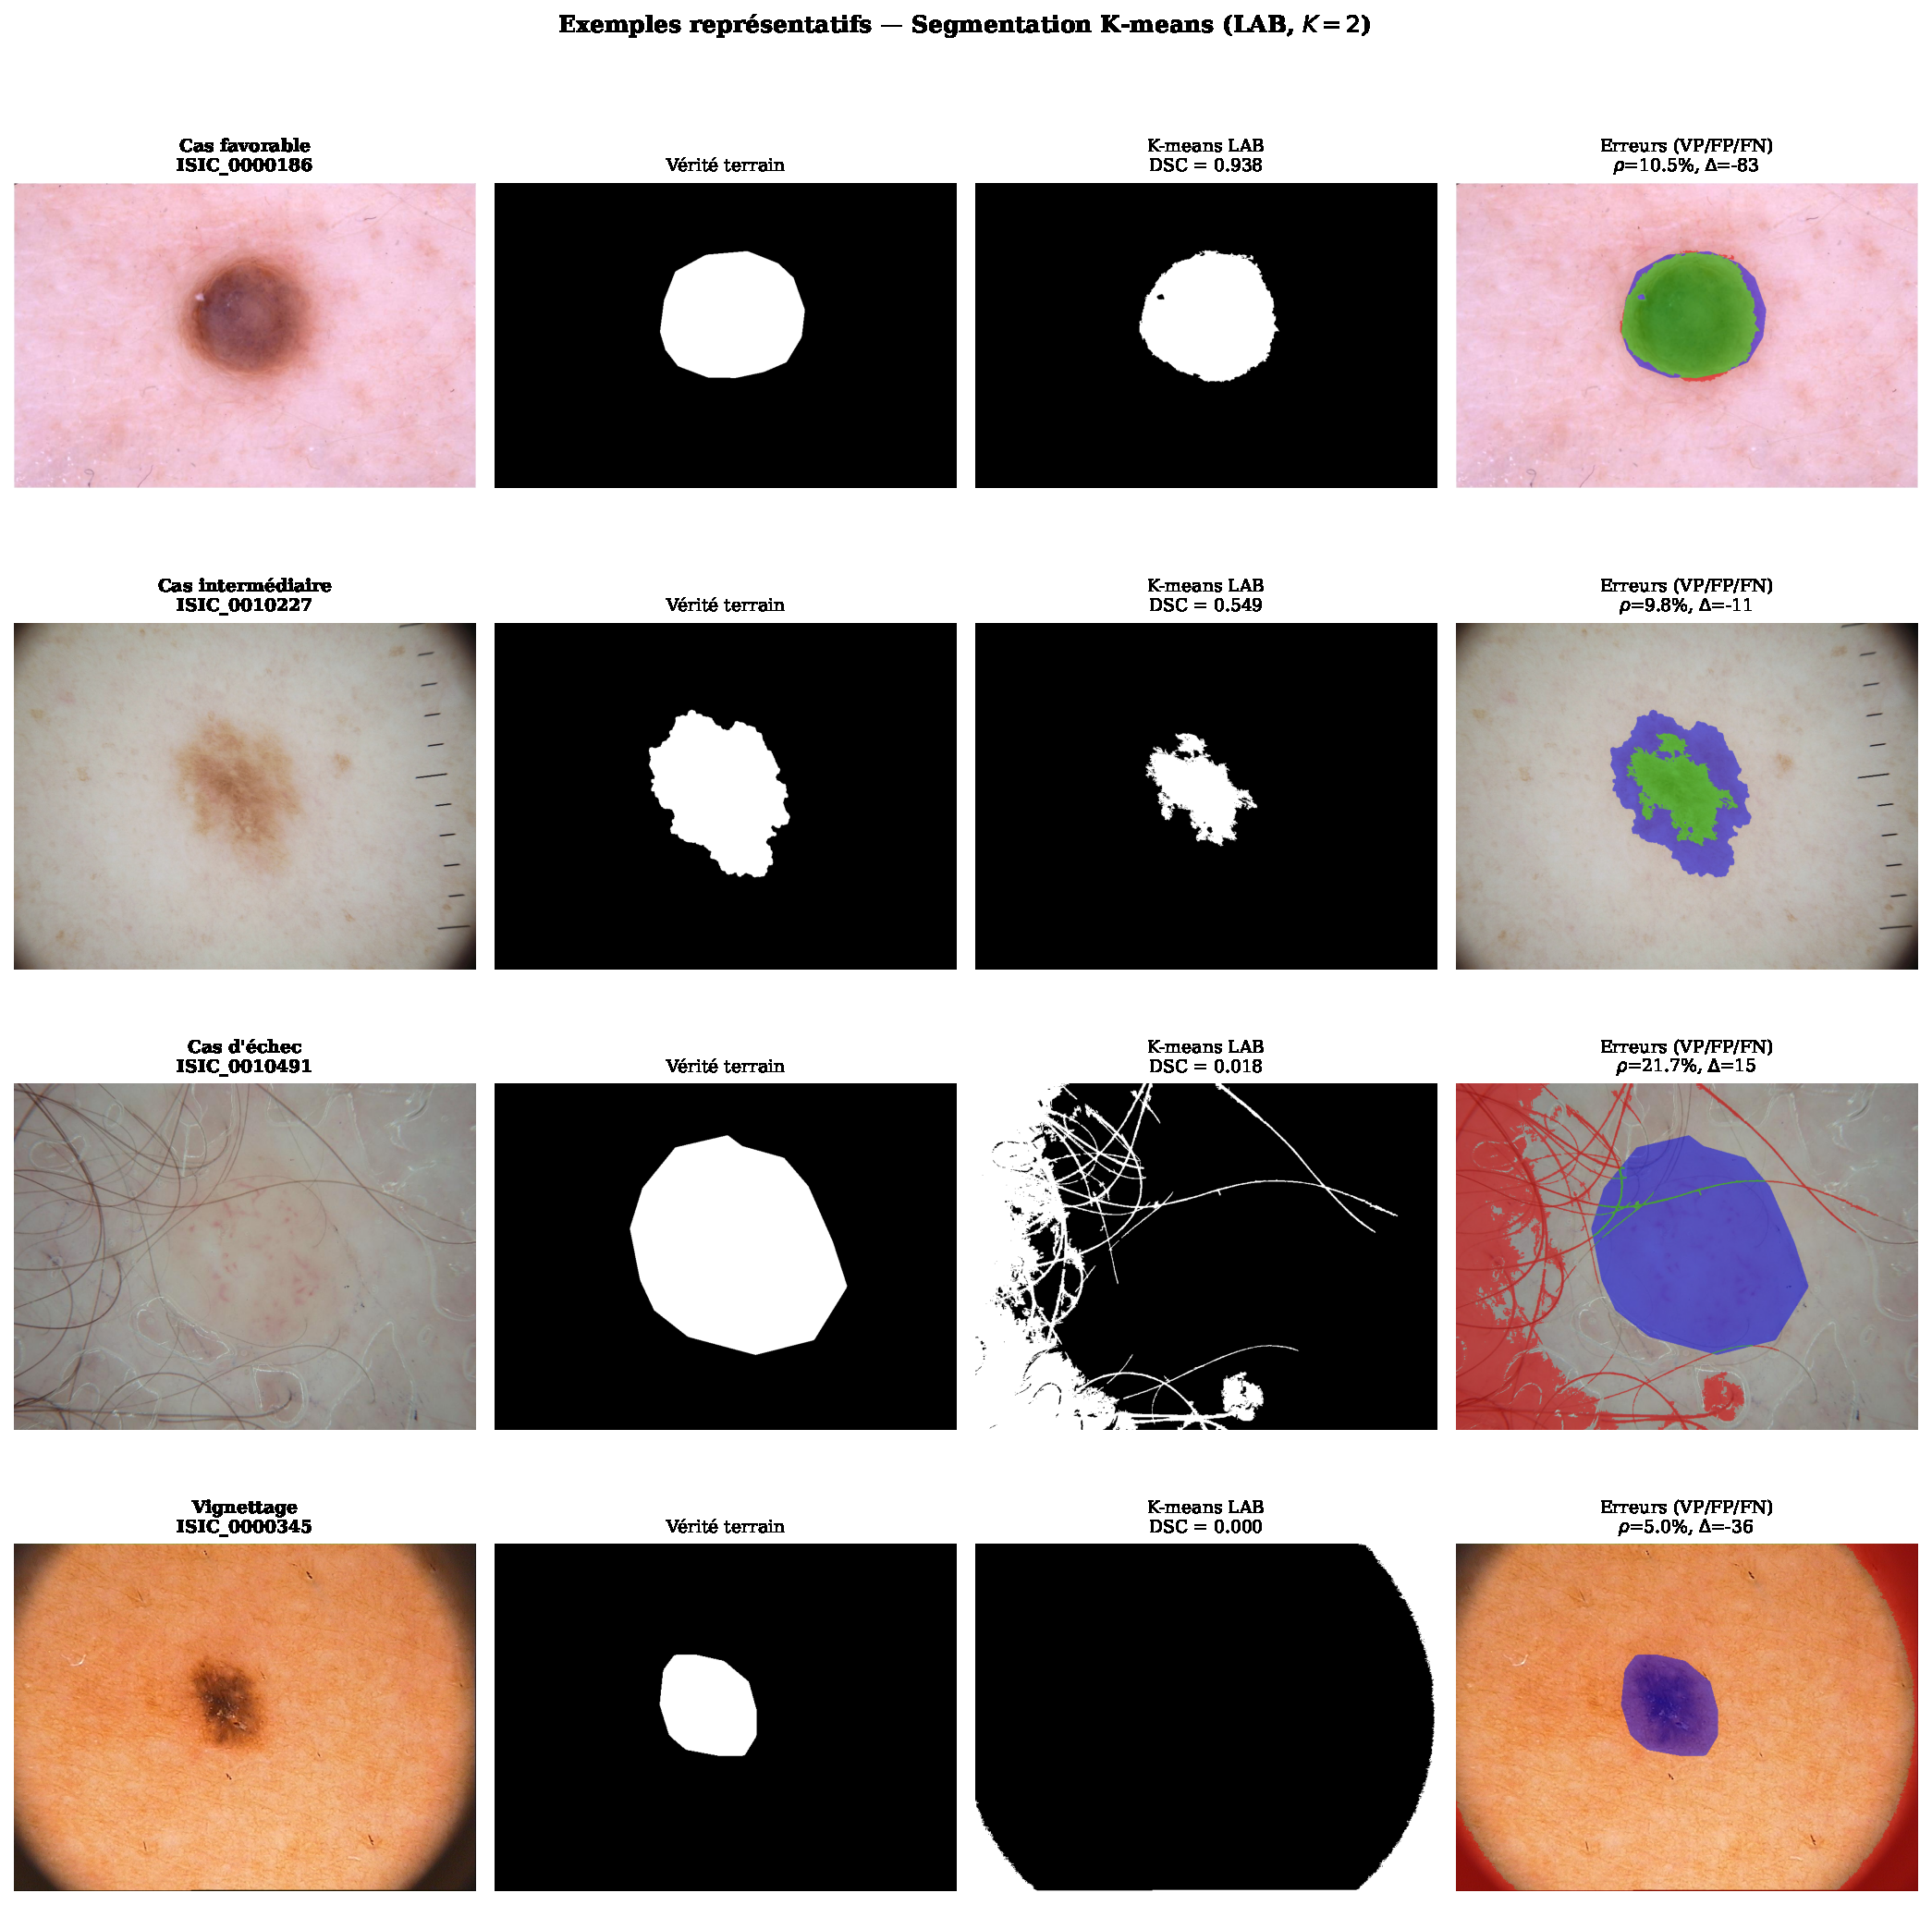
\includegraphics[width=\textwidth]{fig_kmeans_qualitative.pdf}
\caption{Exemples représentatifs de la segmentation par $K$-means (LAB, $K = 2$). De haut en bas~: cas favorable (DSC~$= 0{,}938$), cas intermédiaire (DSC~$= 0{,}549$), cas d'échec sans vignettage (DSC~$= 0{,}018$) et cas d'échec par vignettage (DSC~$= 0{,}000$). La colonne de droite superpose les erreurs~: vert~= vrais positifs, rouge~= faux positifs, bleu~= faux négatifs.}
\label{fig:kmeans_qualitative}
\end{figure}

\subsubsection{Comparaison des espaces colorimétriques}

Le tableau~\ref{tab:kmeans_couleurs} présente les performances agrégées des quatre variantes colorimétriques sur l'ensemble des 900~images, avec $K = 2$ et l'heuristique de luminosité. Un échec est défini comme une segmentation dont le DSC est inférieur à~$0{,}5$.

\begin{table}[H]
\centering
\caption{Performances des variantes $K$-means par espace colorimétrique ($n = 900$, $K = 2$, heuristique sombre). La meilleure valeur par colonne est indiquée en gras.}
\label{tab:kmeans_couleurs}
\begin{tabular}{l r r r r r}
\toprule
\textbf{Variante} & \textbf{DSC} & \textbf{IoU} & \textbf{Accuracy} & \textbf{Précision} & \textbf{Échecs (\%)} \\
\midrule
RGB           & $0{,}580 \pm 0{,}365$ & $0{,}493 \pm 0{,}334$ & $0{,}827 \pm 0{,}170$ & $0{,}707 \pm 0{,}432$ & 31{,}1 \\
RGB + spatial & $0{,}576 \pm 0{,}368$ & $0{,}490 \pm 0{,}336$ & $0{,}825 \pm 0{,}169$ & $0{,}698 \pm 0{,}435$ & 31{,}7 \\
\textbf{LAB}  & $\mathbf{0{,}623 \pm 0{,}356}$ & $\mathbf{0{,}537 \pm 0{,}329}$ & $\mathbf{0{,}840 \pm 0{,}172}$ & $\mathbf{0{,}745 \pm 0{,}416}$ & \textbf{26{,}2} \\
HSV           & $0{,}556 \pm 0{,}367$ & $0{,}471 \pm 0{,}340$ & $0{,}783 \pm 0{,}220$ & $0{,}647 \pm 0{,}425$ & 36{,}3 \\
\bottomrule
\end{tabular}
\end{table}

La figure~\ref{fig:kmeans_boxplot} illustre la distribution des DSC pour chaque variante. L'espace CIE~LAB obtient les meilleures performances sur toutes les métriques (DSC~$= 0{,}623 \pm 0{,}356$), avec un taux d'échec de 26{,}2\%. L'espace RGB natif se situe en deuxième position (DSC~$= 0{,}580$), suivi de RGB+spatial ($0{,}576$) et HSV ($0{,}556$, 36{,}3\% d'échecs). Deux résultats méritent d'être soulignés~:

\begin{figure}[H]
\centering
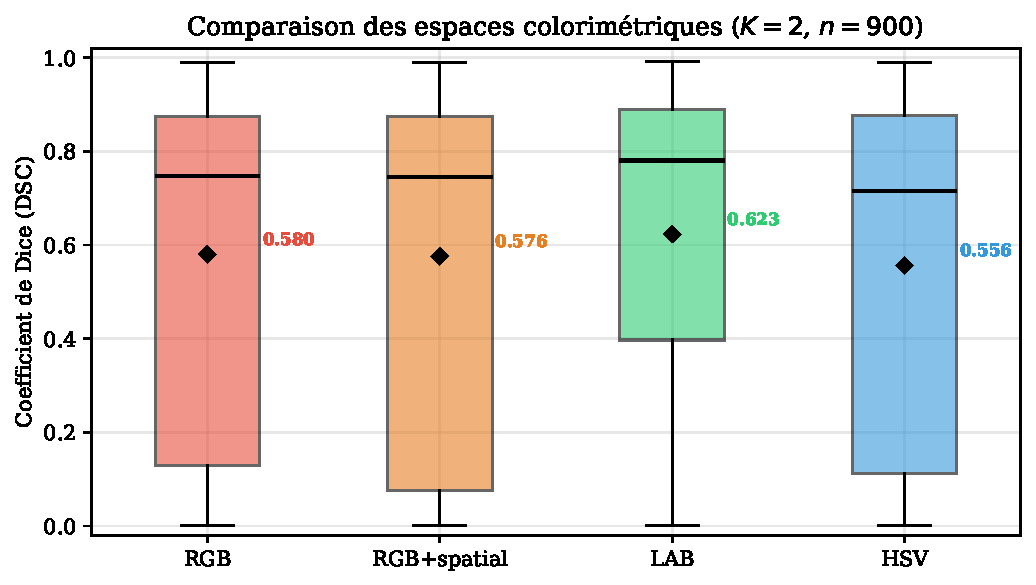
\includegraphics[width=0.75\textwidth]{fig_kmeans_boxplot_variantes.pdf}
\caption{Distribution du DSC pour les quatre variantes colorimétriques ($n = 900$, $K = 2$). Le losange noir indique la moyenne. L'espace LAB domine sur l'ensemble de la distribution, tandis que le HSV présente la plus forte dispersion.}
\label{fig:kmeans_boxplot}
\end{figure}
\begin{itemize}[nosep]
    \item L'\textbf{ajout des coordonnées spatiales} (RGB+spatial) n'améliore pas les performances par rapport au RGB seul ($\Delta\text{DSC} = -0{,}004$). La pondération spatiale ($\alpha = 50$) introduit un biais de position qui pénalise les lésions excentrées sans compenser par une meilleure compacité des clusters.
    \item L'espace \textbf{HSV} est le moins performant, malgré sa séparation théorique entre teinte et luminosité. La circularité de la composante $H$ (discontinuité à $0° \equiv 360°$) perturbe la distance euclidienne utilisée par le $K$-means, engendrant des partitions incohérentes pour les teintes proches du rouge.
\end{itemize}

L'avantage du LAB s'explique par son \textbf{uniformité perceptuelle}~: les distances euclidiennes dans cet espace sont plus fidèles à la perception humaine des différences de couleur, ce qui produit des frontières de partition plus pertinentes pour la séparation lésion/fond. Néanmoins, les écarts entre variantes restent modestes ($\Delta\text{DSC}_{\max} = 0{,}067$) au regard de la variabilité intra-méthode ($\sigma \approx 0{,}36$), ce qui indique que le choix de l'espace colorimétrique ne constitue pas le facteur limitant principal. Notons que le facteur $\alpha = 50$ pour la variante RGB+spatial a été fixé empiriquement sans analyse de sensibilité~: le résultat négatif de cette variante pourrait être partiellement imputable à un choix sous-optimal de~$\alpha$.

\paragraph{Coût computationnel.} Le temps de calcul moyen est de $\sim 0{,}5$~s par image sur CPU, soit \textbf{7~minutes} pour les 900~images --- un avantage pratique notable par rapport aux architectures supervisées nécessitant un GPU.

\subsubsection{Analyse par sous-groupes de difficulté}

Les performances sont fortement conditionnées par la taille de la lésion et le contraste lésion/fond, comme l'illustre la figure~\ref{fig:kmeans_scatter}. Pour la variante LAB, le DSC moyen passe de $0{,}146$ pour les petites lésions ($\rho < 5\%$) à $0{,}728$ pour les grandes ($\rho > 10\%$), et de $0{,}338$ pour les images à faible contraste ($|\Delta| < 20$) à $0{,}820$ pour celles à contraste élevé ($|\Delta| \geq 50$).

\begin{figure}[H]
\centering
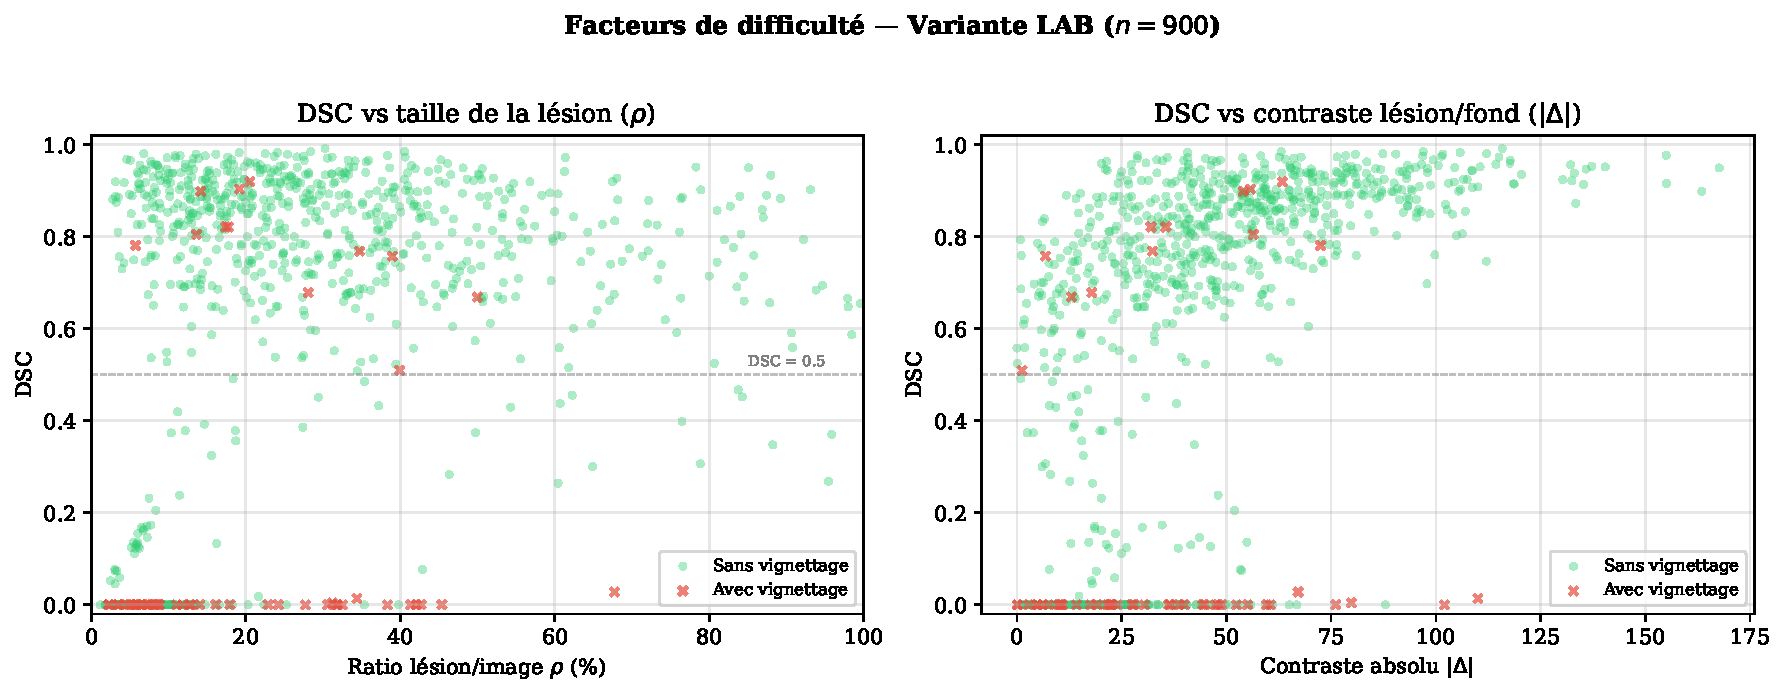
\includegraphics[width=\textwidth]{fig_kmeans_scatter_difficulte.pdf}
\caption{DSC en fonction de la taille de la lésion ($\rho$, à gauche) et du contraste lésion/fond ($|\Delta|$, à droite) pour la variante LAB ($n = 900$). Les croix rouges indiquent les images avec vignettage. La ligne horizontale grise marque le seuil d'échec (DSC~$= 0{,}5$).}
\label{fig:kmeans_scatter}
\end{figure}

\paragraph{Effet du vignettage.} La détection heuristique identifie \textbf{52~images} (5{,}8\% du corpus) présentant un vignettage. Sur ces images, le DSC moyen chute à $0{,}180$ (contre $0{,}650$ hors vignettage), soit une dégradation de $-0{,}470$ points. La bordure sombre est systématiquement absorbée dans le cluster de la lésion, produisant une sur-segmentation massive. Cette limitation structurelle, liée à l'absence de modélisation spatiale, ne peut être résolue par un simple changement d'espace colorimétrique.

\subsubsection{Estimation du nombre optimal de clusters}
\label{subsubsec:resultats_k}

Les trois méthodes d'estimation du $K$ optimal ont été appliquées au sous-ensemble stratifié de 225~images (figure~\ref{fig:kmeans_kstar}). Les résultats divergent radicalement~: le mode est $K^\star = 3$ pour l'Elbow, $K^\star = 2$ pour le Silhouette (90{,}2\% des images) et $K^\star = 6$ pour le BIC. La concordance est \textbf{nulle}~: aucune image ne reçoit le même $K^\star$ par les trois méthodes. Cette divergence reflète la nature différente de chaque critère~:
\begin{itemize}[nosep]
    \item Le \textbf{score de silhouette}, qui évalue la séparabilité effective des clusters, identifie la structure binaire lésion/fond dans 90{,}2\% des cas, confirmant empiriquement l'adéquation du choix $K = 2$.
    \item La \textbf{méthode du coude} détecte systématiquement un troisième cluster ($K^\star = 3$ dans 93{,}3\% des cas), correspondant vraisemblablement à une classe intermédiaire (zones de transition, artefacts) qui réduit l'inertie sans correspondre à une structure sémantiquement pertinente.
    \item Le \textbf{BIC} favorise $K^\star = 6$ (88{,}4\%), traduisant une modélisation fine de la texture cutanée (pores, variations locales de pigmentation) plutôt qu'une partition sémantique. Le GMM, plus flexible que le $K$-means (matrices de covariance complètes), est davantage sujet au sur-ajustement des variations non pertinentes pour la segmentation.
\end{itemize}

Ce résultat constitue en soi un apport méthodologique~: il illustre le \textbf{décalage entre l'optimisation d'un critère de clustering} (ajustement statistique aux données) \textbf{et l'objectif applicatif} (segmentation sémantique). Le $K$ optimal au sens d'un critère statistique n'est pas nécessairement celui qui produit la meilleure segmentation. La figure~\ref{fig:kmeans_kstar} illustre cette divergence.

\begin{figure}[H]
\centering
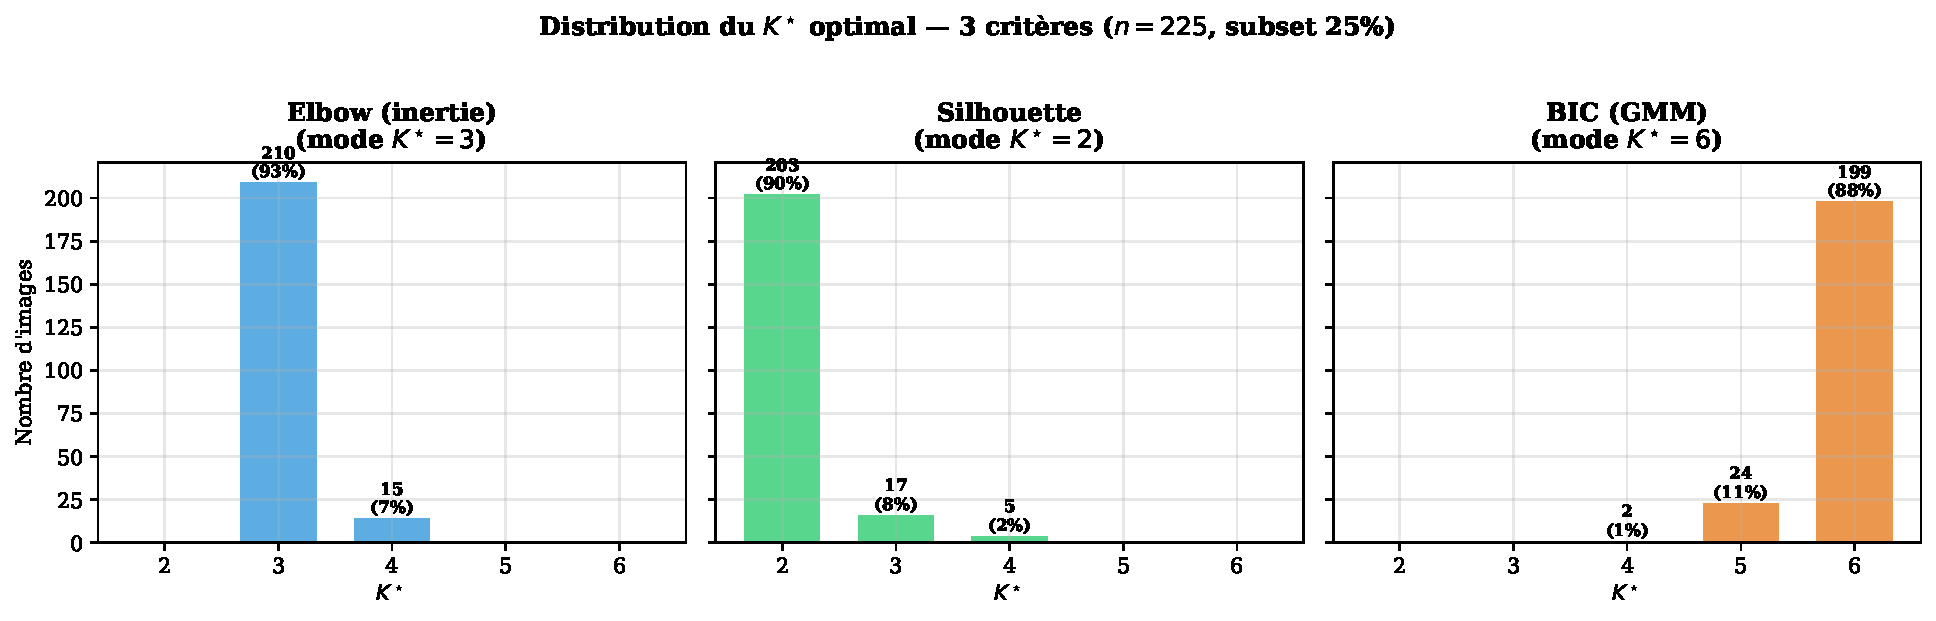
\includegraphics[width=\textwidth]{fig_kmeans_kstar_distribution.pdf}
\caption{Distribution du $K^\star$ optimal estimé par trois critères ($n = 225$). Le mode diffère radicalement~: $K^\star = 3$ (Elbow), $K^\star = 2$ (Silhouette) et $K^\star = 6$ (BIC). Aucune image ne reçoit le même $K^\star$ par les trois méthodes.}
\label{fig:kmeans_kstar}
\end{figure}

\subsubsection{Étude d'ablation~: $K \times$ règle d'assignation}
\label{subsubsec:ablation_kmeans}

Le tableau~\ref{tab:k_grid} présente les résultats de la grille $2 \times 2$ sur le sous-ensemble de 225~images. Le $K$ adaptatif est déterminé par le score de silhouette, retenu comme le critère le plus pertinent d'après l'analyse précédente.

\begin{table}[H]
\centering
\caption{Grille d'ablation $K \times$ assignation (espace RGB, $n = 225$, subset stratifié 25\%). La meilleure configuration est indiquée en gras.}
\label{tab:k_grid}
\begin{tabular}{l r r r r}
\toprule
\textbf{Configuration} & \textbf{DSC} & \textbf{IoU} & \textbf{Accuracy} & \textbf{Échecs} \\
\midrule
$K = 2$, sombre            & $\mathbf{0{,}576 \pm 0{,}357}$ & $\mathbf{0{,}484 \pm 0{,}324}$ & $\mathbf{0{,}823 \pm 0{,}159}$ & \textbf{69} \\
$K = 2$, centralité        & $0{,}463 \pm 0{,}353$ & $0{,}375 \pm 0{,}325$ & $0{,}527 \pm 0{,}343$ & 114 \\
$K$ adaptatif, sombre       & $0{,}570 \pm 0{,}355$ & $0{,}478 \pm 0{,}323$ & $0{,}823 \pm 0{,}168$ & 72 \\
$K$ adaptatif, centralité   & $0{,}458 \pm 0{,}351$ & $0{,}370 \pm 0{,}324$ & $0{,}526 \pm 0{,}340$ & 116 \\
\bottomrule
\end{tabular}
\end{table}

La décomposition des effets marginaux (en $\Delta$DSC par rapport à la baseline $K = 2$ sombre) met en évidence deux résultats~:
\begin{itemize}[nosep]
    \item \textbf{Effet de la règle d'assignation} (centralité vs.\ sombre, à $K = 2$)~: $\Delta\text{DSC} = -0{,}113$. La centralité dégrade fortement les performances (taux d'échec de 50{,}7\%). Malgré un centrage moyen des lésions, le fond reste majoritaire même dans le quart central de l'image, et est fréquemment assigné à tort à la classe lésion.
    \item \textbf{Effet du $K$ adaptatif} (à heuristique sombre fixée)~: $\Delta\text{DSC} = -0{,}006$. Le $K$ adaptatif n'apporte aucune amélioration mesurable~: puisque 90{,}2\% des images reçoivent $K^\star = 2$ par silhouette, le $K$ adaptatif se réduit de facto à $K = 2$ dans l'écrasante majorité des cas.
\end{itemize}

\subsubsection{Synthèse}
\label{subsubsec:discussion_kmeans}

L'ensemble des résultats valide empiriquement la configuration $K = 2$ avec heuristique de luminosité dans l'espace LAB comme le meilleur compromis pour la segmentation non supervisée. L'estimation data-driven du $K$ optimal confirme l'adéquation de la structure binaire (silhouette~$\to K = 2$ dans 90{,}2\% des cas), et la règle d'assignation par le cluster le plus sombre ($+0{,}113$ DSC vs.\ centralité) s'appuie sur l'observation que 96{,}1\% des lésions sont plus sombres que le fond. Néanmoins, le $K$-means reste fondamentalement limité par l'absence de modélisation spatiale (vulnérabilité au vignettage, DSC~$= 0{,}180$), l'hypothèse de clusters sphériques, et un taux d'échec structurel $\geq 26\%$ concentré sur les petites lésions ($\rho < 5\%$, DSC~$= 0{,}146$) et le faible contraste ($|\Delta| < 20$, DSC~$= 0{,}338$). Ces limitations motivent le recours à des architectures supervisées.

\subsection{Segmentation par CNN sur patches}
\label{subsec:resultats_cnn_patch}

La figure~\ref{fig:cnn_qualitative} illustre trois cas représentatifs de la segmentation par CNN patch ($P = 32$), mettant en évidence la carte de probabilités intermédiaire et le masque final après post-traitement. L'analyse quantitative détaillée suit.

\begin{figure}[H]
\centering
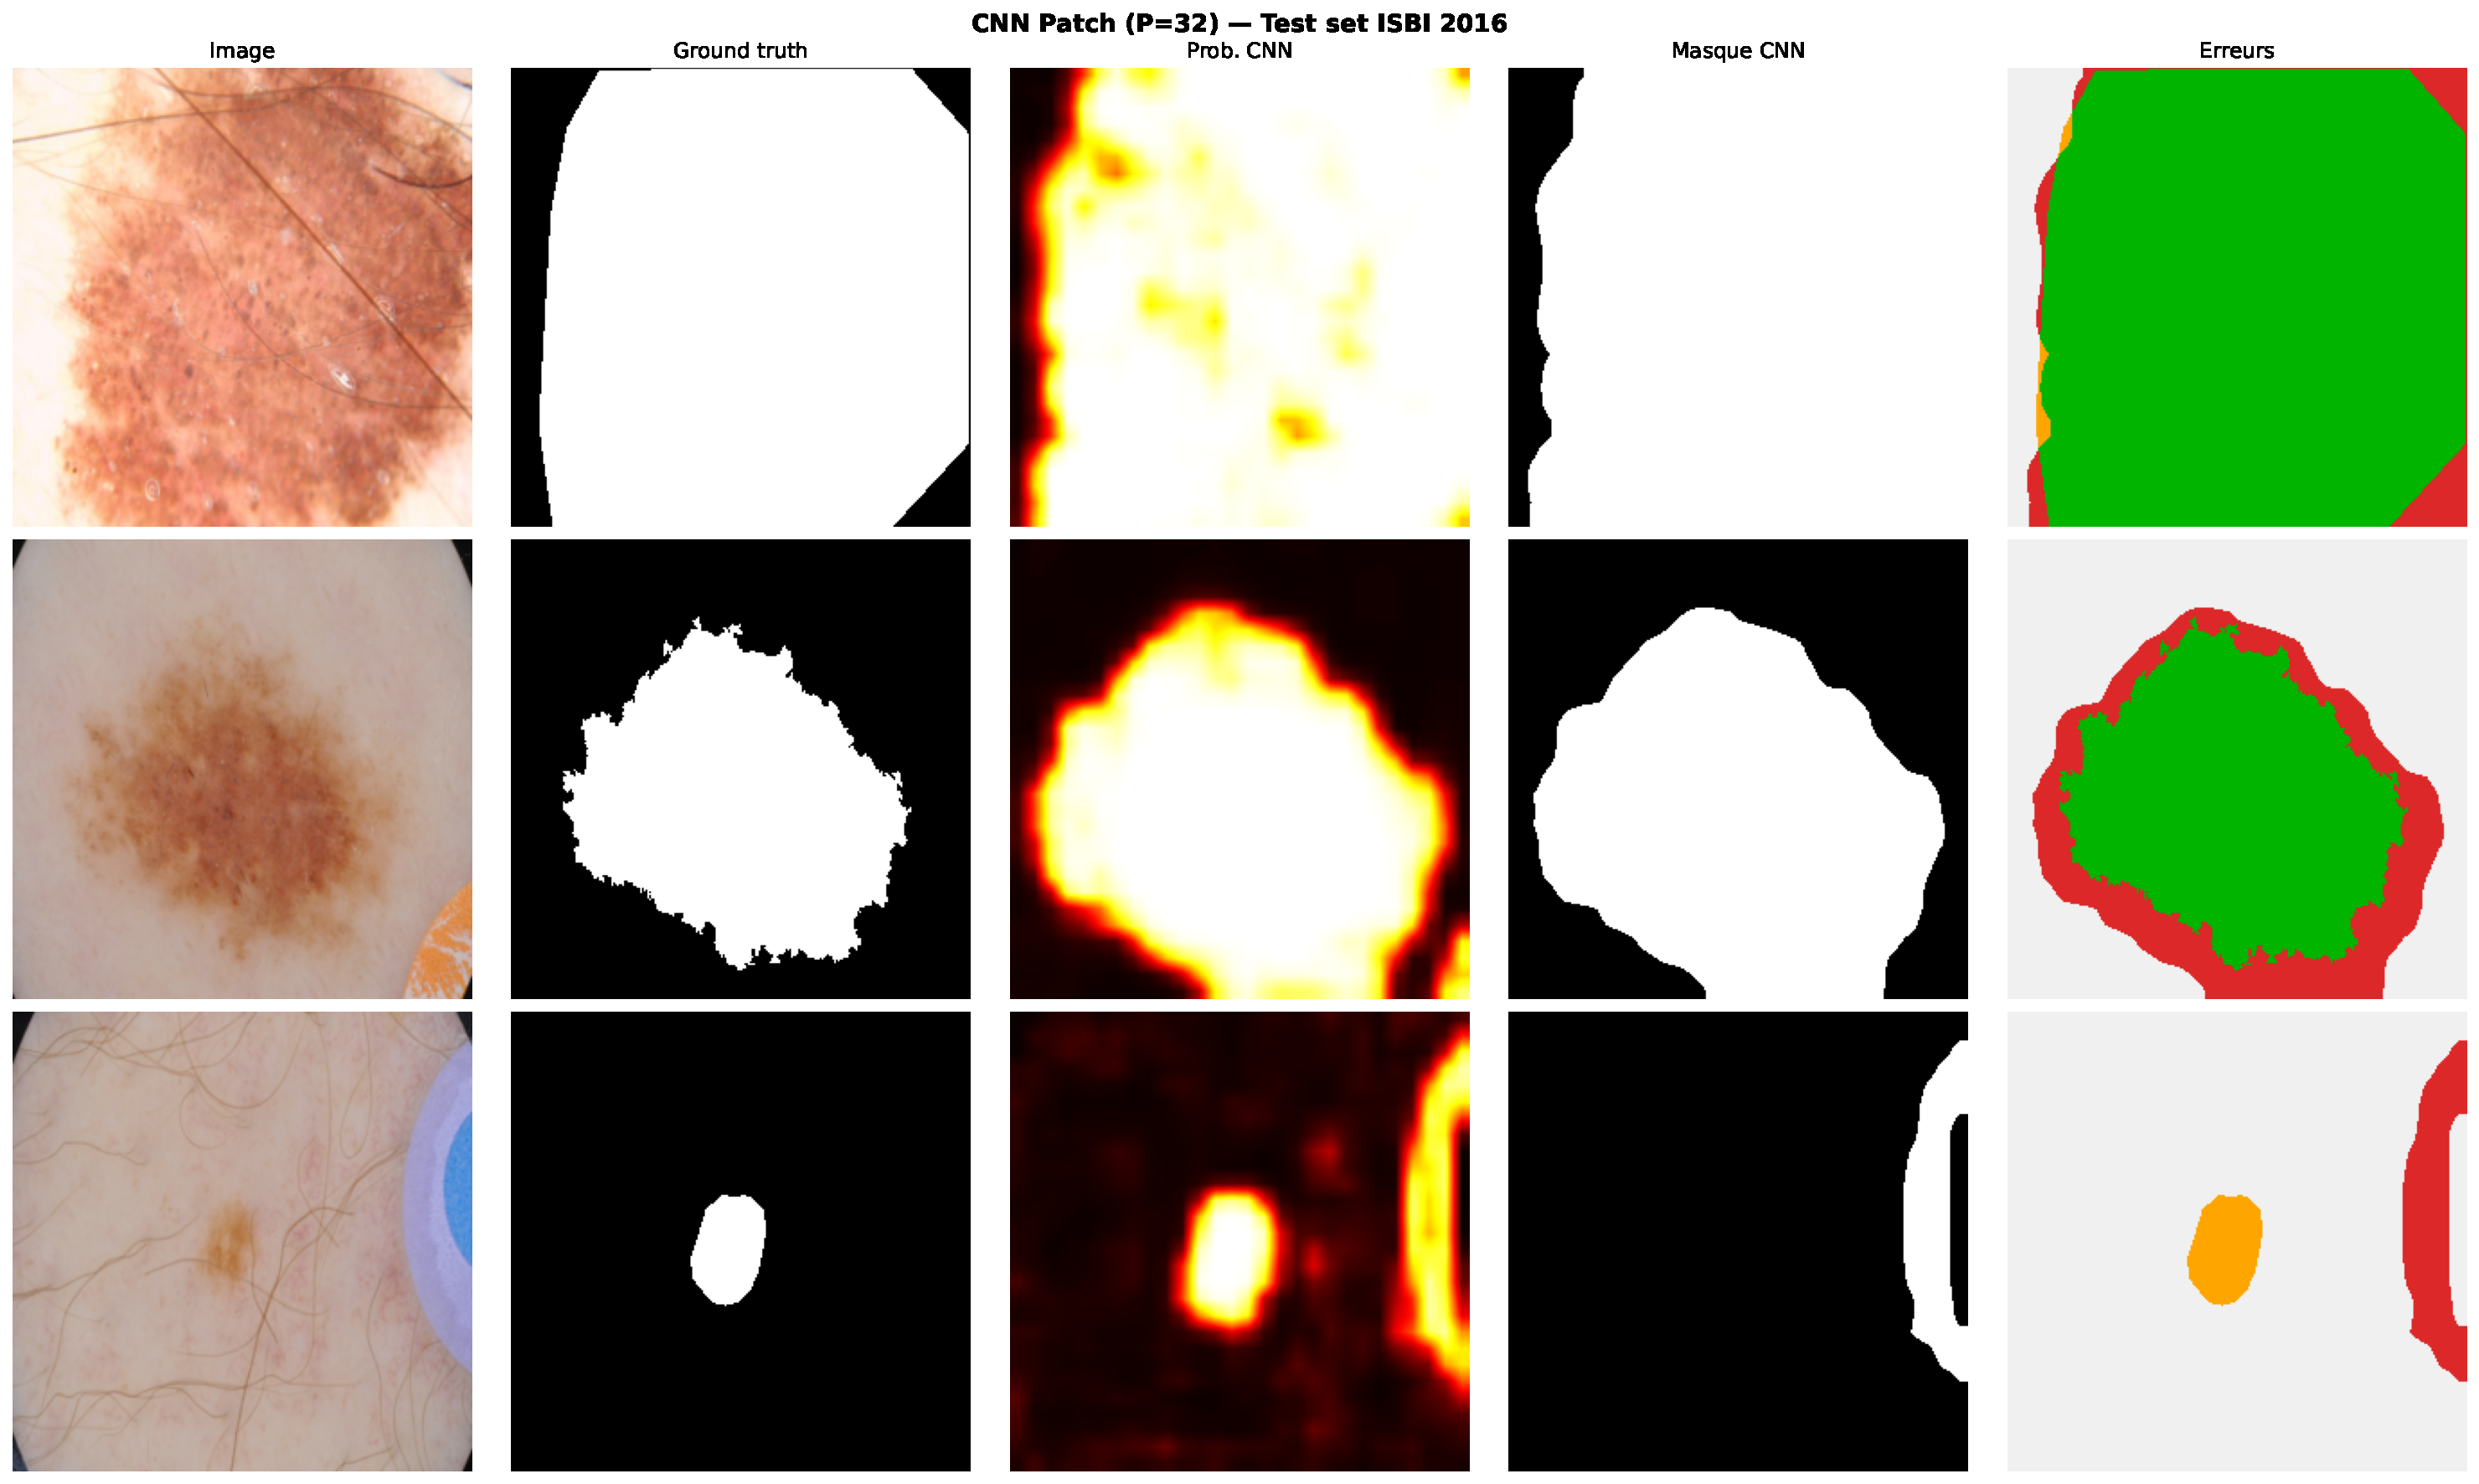
\includegraphics[width=\textwidth]{fig_cnn_patch_qualitative.pdf}
\caption{Exemples représentatifs de la segmentation par CNN patch ($P = 32$). De haut en bas~: meilleur cas, cas médian, pire cas. Colonnes~: image originale, masque de référence, carte de probabilités du CNN (colormap \emph{hot}), masque prédit, carte d'erreurs (vert~= VP, rouge~= FP, orange~= FN). La carte de probabilités révèle la structure de la grille d'inférence et les zones de faux positifs typiques (artefacts sombres).}
\label{fig:cnn_qualitative}
\end{figure}

\subsubsection{Convergence de l'entraînement}

Le modèle $P = 48$ converge en \textbf{13 epochs} (sur 30 maximum), l'early stopping (patience $= 5$) se déclenchant à l'epoch 18 avec restauration des meilleurs poids. L'accuracy de classification des patches atteint $91{,}2\%$ en validation, avec un écart train/validation faible ($\Delta\text{acc} = 0{,}02$), indiquant une absence de sur-apprentissage. Le modèle $P = 32$, en revanche, utilise les 30 epochs sans déclenchement de l'early stopping, ce qui suggère une convergence plus lente liée au champ réceptif plus restreint~; la \texttt{val\_loss} reste néanmoins stable sur les dernières epochs, excluant un sur-apprentissage significatif. Le temps d'entraînement total est de $\sim 12$ minutes sur GPU NVIDIA Tesla T4 (16~Go VRAM), soit un temps comparable à celui du U-Net baseline.

\subsubsection{Étude d'ablation de la taille de patch}

Le tableau~\ref{tab:cnn_patch_ablation} présente les résultats de l'ablation sur la taille du patch $P$. Chaque modèle est évalué sur les 180~images de validation par inférence en fenêtre glissante, avec post-traitement par plus grande composante connexe.

\begin{table}[H]
\centering
\caption{Étude d'ablation de la taille de patch $P$ pour le CNN patch-based (validation, $n = 180$). La meilleure configuration est indiquée en gras.}
\label{tab:cnn_patch_ablation}
\footnotesize
\begin{tabular}{l r r r r r r r r}
\toprule
\textbf{Patch $P$} & \textbf{Params} & \textbf{Ep.} & \textbf{DSC} & \textbf{IoU} & \textbf{Préc.} & \textbf{Rappel} & \textbf{Acc.\ patch} & \textbf{Éch.} \\
\midrule
$\mathbf{32 \times 32}$ & \textbf{147\,745} & \textbf{30} & $\mathbf{0{,}765 \pm 0{,}151}$ & $\mathbf{0{,}639 \pm 0{,}161}$ & $\mathbf{0{,}685}$ & $0{,}930$ & \textbf{0{,}915} & \textbf{8} \\
$48 \times 48$ & 147\,745 & 18 & $0{,}732 \pm 0{,}153$ & $0{,}596 \pm 0{,}156$ & $0{,}634$ & $0{,}930$ & 0{,}912 & 10 \\
$64 \times 64$ & 147\,745 & 11 & $0{,}707 \pm 0{,}138$ & $0{,}562 \pm 0{,}144$ & $0{,}603$ & $0{,}933$ & 0{,}911 & 9 \\
\bottomrule
\end{tabular}
\end{table}

Le résultat le plus notable est la \textbf{relation inverse} entre taille de patch et performance de segmentation~: le patch le plus petit ($P = 32$) obtient le meilleur DSC ($0{,}765$), tandis que le plus grand ($P = 64$) est le moins performant ($0{,}707$, $\Delta = -5{,}8$ pts). Ce résultat, a priori contre-intuitif, s'explique par deux mécanismes complémentaires~:

\begin{enumerate}[nosep]
    \item \textbf{Dilution du signal discriminant.} Un patch de $64 \times 64$ sur une image de $256 \times 256$ couvre $6{,}25\%$ de l'image. Pour les pixels situés près des bords de la lésion, une proportion croissante du patch est occupée par du fond non informatif, ce qui dilue les motifs de texture pertinents pour la classification.
    \item \textbf{Résolution de la grille d'inférence.} À stride $s$ comparable, un petit patch produit davantage de positions valides ($N = 28^2 = 784$ pour $P = 32$ vs $N = 25^2 = 625$ pour $P = 64$), ce qui réduit les erreurs d'interpolation lors du redimensionnement de la grille $G$ (équation~\ref{eq:grid}) à la résolution originale.
\end{enumerate}

L'accuracy de classification des patches est quasi identique pour les trois tailles ($\approx 0{,}91$), confirmant que le CNN apprend des représentations utiles quelle que soit la taille du patch. L'écart de performance en segmentation provient donc principalement de la procédure d'inférence, et non de la qualité intrinsèque du classifieur.

On note également que le nombre d'epochs de convergence \textbf{décroît} avec la taille du patch (30, 18, 11), ce qui suggère que les patches plus grands, contenant davantage d'information redondante, sont plus faciles à classifier mais moins discriminants pour la segmentation fine.

\subsubsection{Compromis précision/rappel}

Le CNN patch présente un comportement diamétralement opposé à celui du $K$-means en termes de compromis précision/rappel. Là où le $K$-means est \textbf{conservateur} (précision $> $ rappel, section~\ref{subsec:resultats_kmeans}), le CNN patch est \textbf{agressif}~: le rappel moyen ($0{,}930$) est nettement supérieur à la précision ($0{,}685$). Autrement dit, le CNN détecte la quasi-totalité des pixels lésionnels mais produit un nombre important de faux positifs.

Ce comportement s'explique par le champ réceptif local du CNN~: un patch de peau sombre (ombre, poil, bordure de loupe) peut être localement indistinguable d'un patch de lésion. Le CNN, n'ayant accès qu'au voisinage immédiat, classe ces patches comme « lésion » par excès de prudence. Le post-traitement par composante connexe corrige partiellement ce biais (précision $+0{,}024$), mais ne peut pas éliminer les faux positifs \emph{adjacents} à la lésion. Le U-Net, en revanche, bénéficie d'un contexte global qui lui permet de lever ces ambiguïtés.

\subsubsection{Impact du post-traitement}

Le post-traitement par conservation de la plus grande composante connexe apporte un gain modeste mais cohérent. Le tableau~\ref{tab:cnn_pp} présente l'impact pour le modèle retenu ($P = 32$) sur les 180~images de validation.

\begin{table}[H]
\centering
\caption{Impact du post-traitement (plus grande composante connexe) sur la validation ($n = 180$, $P = 32$).}
\label{tab:cnn_pp}
\begin{tabular}{l r r r}
\toprule
\textbf{Métrique} & \textbf{Sans PP} & \textbf{Avec PP} & \textbf{$\Delta$} \\
\midrule
DSC       & $0{,}751 \pm 0{,}142$ & $0{,}765 \pm 0{,}151$ & $+0{,}014$ \\
IoU       & $0{,}619 \pm 0{,}163$ & $0{,}639 \pm 0{,}161$ & $+0{,}019$ \\
Accuracy  & $0{,}867 \pm 0{,}109$ & $0{,}875 \pm 0{,}117$ & $+0{,}008$ \\
Precision & $0{,}662 \pm 0{,}180$ & $0{,}685 \pm 0{,}170$ & $+0{,}024$ \\
Recall    & $0{,}942 \pm 0{,}132$ & $0{,}930 \pm 0{,}174$ & $-0{,}012$ \\
\midrule
Échecs (DSC $< 0{,}5$) & 14 & 8 & $-6$ \\
\bottomrule
\end{tabular}
\end{table}

Le mécanisme est le suivant~: la suppression des composantes secondaires élimine les \textbf{faux positifs isolés} (gain en précision, $+0{,}024$) mais peut, dans de rares cas, supprimer de petites régions lésionnelles disjointes (perte en rappel, $-0{,}012$). Le bilan net est positif sur le DSC ($+0{,}014$) et réduit le nombre d'échecs de 14 à 8. Ce gain est plus modeste que celui observé pour le $K$-means (où le post-traitement corrige les faux positifs de vignettage), car le CNN patch produit des faux positifs plus souvent \emph{adjacents} à la lésion que \emph{isolés}.

\subsubsection{Évaluation sur le jeu de test officiel}

Le meilleur modèle ($P = 32$) est évalué sur le jeu de test officiel ISBI~2016 (379~images), identique à celui utilisé pour l'évaluation du U-Net (section~\ref{subsec:final_model}). Les résultats globaux et par sous-groupes de taille sont présentés dans le tableau~\ref{tab:cnn_test}.

\begin{table}[H]
\centering
\caption{CNN patch ($P = 32$)~: résultats sur le test set ISBI~2016 ($n = 379$), global et par sous-groupe de taille.}
\label{tab:cnn_test}
\begin{tabular}{l r r r r r}
\toprule
\textbf{Sous-groupe} & \textbf{$n$} & \textbf{DSC} & \textbf{IoU} & \textbf{Accuracy} & \textbf{Échecs} \\
\midrule
Global             & 379 & $0{,}760 \pm 0{,}175$ & $0{,}639 \pm 0{,}184$ & $0{,}868 \pm 0{,}129$ & 29 \\
\midrule
Petites ($\rho < 5\%$)     & 40  & $0{,}590 \pm 0{,}250$ & $0{,}455 \pm 0{,}214$ & $0{,}873 \pm 0{,}124$ & 9 \\
Moyennes ($5\% \leq \rho < 10\%$) & 47  & $0{,}708 \pm 0{,}184$ & $0{,}572 \pm 0{,}177$ & $0{,}862 \pm 0{,}108$ & 6 \\
Grandes ($\rho \geq 10\%$)  & 292 & $0{,}792 \pm 0{,}144$ & $0{,}675 \pm 0{,}162$ & $0{,}868 \pm 0{,}133$ & 14 \\
\bottomrule
\end{tabular}
\end{table}

\paragraph{Analyse par sous-groupes.} Afin de garantir une comparaison équitable, le $K$-means (LAB, $K = 2$, heuristique sombre) est également évalué sur les mêmes 379~images de test. Le gradient de performance selon la taille de la lésion est similaire à celui observé sur le train set mais \textbf{considérablement atténué} avec le CNN. Le tableau~\ref{tab:cnn_vs_kmeans_subgroups} met en regard les deux approches par sous-groupe.

\begin{table}[H]
\centering
\caption{Comparaison $K$-means LAB vs CNN patch ($P = 32$) par sous-groupe de taille (test set, $n = 379$).}
\label{tab:cnn_vs_kmeans_subgroups}
\begin{tabular}{l r r r}
\toprule
\textbf{Sous-groupe} & \textbf{$K$-means LAB} & \textbf{CNN Patch} & \textbf{$\Delta$ DSC} \\
\midrule
Petites ($\rho < 5\%$)     & $0{,}197$ & $0{,}590$ & $+0{,}393$ \\
Moyennes ($5\% \leq \rho < 10\%$) & $0{,}411$ & $0{,}708$ & $+0{,}297$ \\
Grandes ($\rho \geq 10\%$)  & $0{,}748$ & $0{,}792$ & $+0{,}044$ \\
\bottomrule
\end{tabular}
\end{table}

Le gain du CNN patch est d'autant plus important que la lésion est petite~: $+0{,}393$ DSC pour les petites lésions, contre seulement $+0{,}044$ pour les grandes. Ce résultat s'explique par le fait que le $K$-means échoue sur les petites lésions par \textbf{déséquilibre de classes} (les pixels lésionnels sont noyés dans le cluster du fond), un problème que le CNN patch évite grâce à l'échantillonnage équilibré et à la supervision. En revanche, pour les grandes lésions à contraste élevé, le $K$-means produit déjà des segmentations raisonnables, et le gain marginal de la supervision est plus limité.

\begin{figure}[H]
\centering
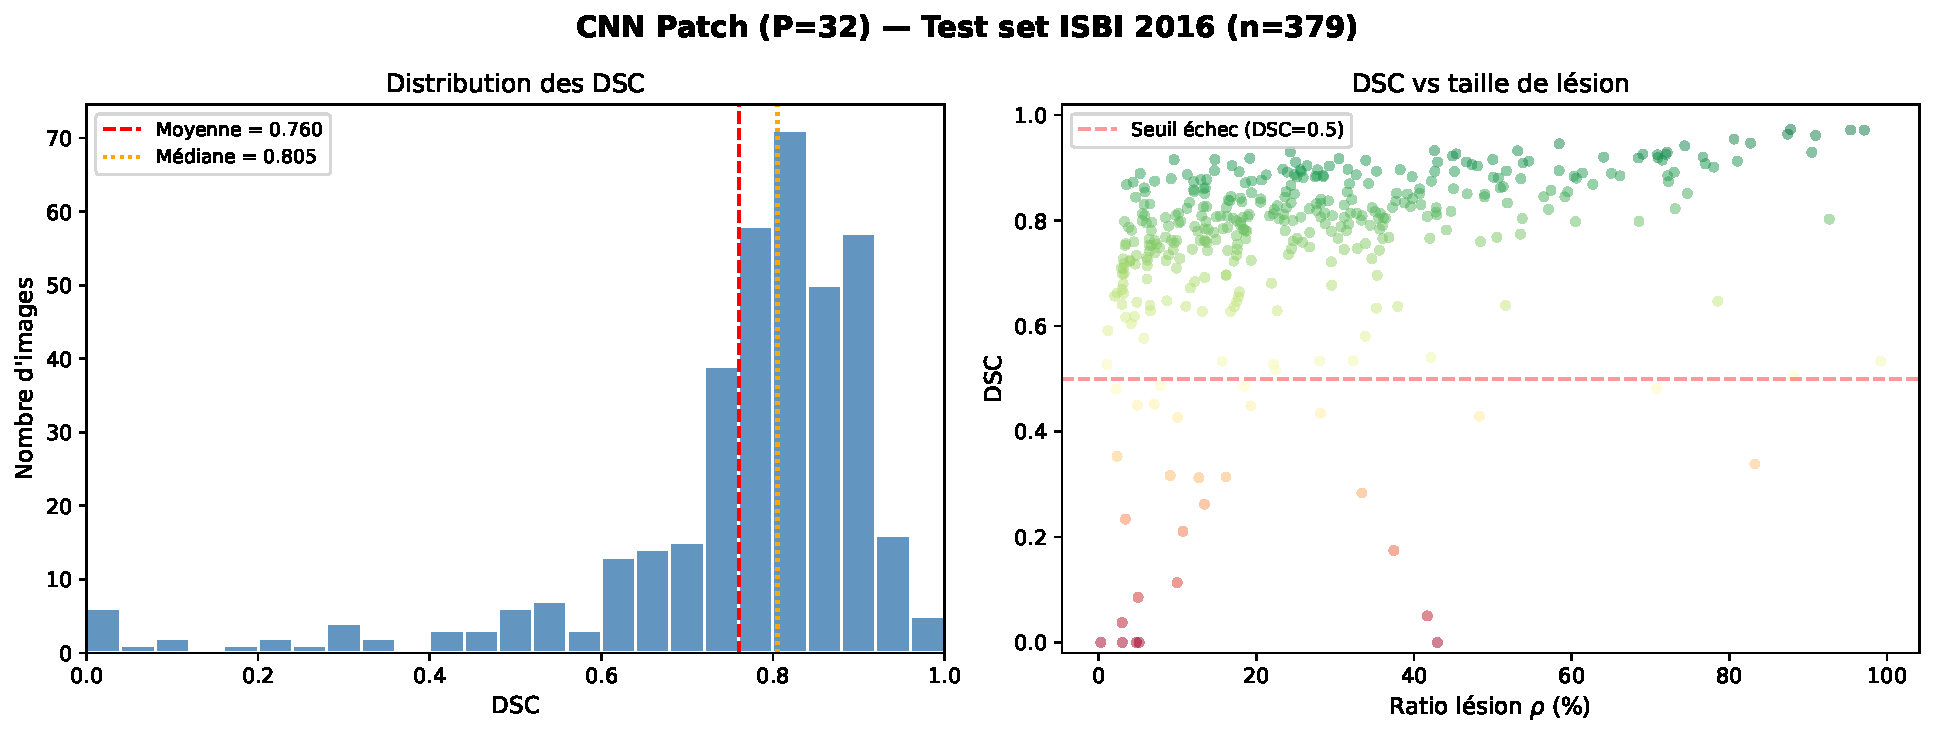
\includegraphics[width=\textwidth]{fig_cnn_patch_distribution.pdf}
\caption{Distribution des DSC sur le test set ISBI~2016 ($n = 379$). À gauche~: histogramme avec moyenne (rouge) et médiane (orange). À droite~: DSC en fonction du ratio de lésion $\rho$, coloré par DSC. La ligne horizontale marque le seuil d'échec (DSC~$= 0{,}5$).}
\label{fig:cnn_distribution}
\end{figure}

\paragraph{Taux d'échec.} Le CNN patch produit 29 échecs (DSC~$< 0{,}5$, soit 7{,}7\% du test set), contre 23{,}7\% pour le $K$-means LAB évalué sur le même test set. Parmi ces 29 échecs, 9 concernent les petites lésions ($\rho < 5\%$, $n = 40$, taux d'échec de 22{,}5\%), confirmant que cette catégorie reste la plus difficile même avec supervision.

\paragraph{Coût computationnel.} Le temps d'inférence moyen est de $0{,}19$~s/image pour le CNN patch ($P = 32$, stride $= 8$, 784 évaluations) sur GPU Tesla T4. Ce temps est inférieur à celui du $K$-means ($0{,}48$~s/image), mais la comparaison est trompeuse~: le CNN s'exécute sur GPU tandis que le $K$-means tourne sur CPU. Le coût réel du CNN réside dans le nombre d'évaluations ($\sim 784$ par image), qui croîtrait quadratiquement avec la résolution d'entrée ou un stride plus fin.

\subsubsection{Discussion}

Le CNN patch-based se positionne, comme attendu, entre le $K$-means et le U-Net (DSC test~$= 0{,}760$ vs $0{,}648$ et $0{,}882$ respectivement, tous évalués sur le même test set ISBI~2016). Deux apports principaux expliquent le gain par rapport au $K$-means~: (i)~les \textbf{convolutions apprises} capturent des motifs locaux (gradient de texture, structure de bord) que le clustering sur des vecteurs de couleur bruts ne peut pas exploiter~; (ii)~la \textbf{supervision} permet d'adapter les représentations à la tâche, en s'affranchissant de l'heuristique « cluster sombre = lésion ».

Cependant, l'approche par patches présente trois \textbf{limitations structurelles} qui motivent directement l'adoption du U-Net~:
\begin{enumerate}[nosep]
    \item \textbf{Champ réceptif local}~: le CNN ne voit qu'un patch $P \times P$ ($1{,}6\%$ de l'image pour $P = 32$) et n'a aucun accès au contexte global. Il ne peut pas distinguer un artefact sombre (bordure de loupe, ombre) de la lésion si leurs textures locales sont similaires, d'où le faible ratio précision/rappel ($0{,}685/0{,}930$).
    \item \textbf{Absence de cohérence spatiale}~: chaque pixel est classifié indépendamment, produisant des masques bruités aux contours irréguliers, partiellement corrigés par le post-traitement mais sans garantie de continuité. L'architecture encodeur-décodeur du U-Net, avec ses skip connections, permet de recombiner informations locales et globales pour produire des masques spatialement cohérents.
    \item \textbf{Inférence lente}~: la segmentation d'une image nécessite $\sim 784$ évaluations du CNN ($P = 32$, stride $= 8$), contre un seul forward pass pour le U-Net. Bien que le temps absolu soit modeste ($0{,}19$~s), le passage à une résolution plus élevée ou un stride plus fin rendrait cette approche prohibitive.
\end{enumerate}

Ces limitations, inhérentes à l'approche par patches et non à l'architecture du CNN elle-même, justifient le passage à une architecture de segmentation dense (\emph{pixel-wise}) capable de traiter l'image entière en un seul passage.

\subsection{Résultats de la baseline U-Net}
\label{subsec:baseline_unet}

La configuration de base du réseau U-Net (\texttt{f64/d4/skip/BCE+Dice}, 31,4M paramètres) atteint, après 27 epochs d'entraînement, les performances suivantes sur l'ensemble de validation~:
\begin{itemize}[nosep]
    \item \textbf{DSC} $= 0{,}854$~;
    \item \textbf{IoU} $= 0{,}748$~;
    \item \textbf{Pixel Accuracy} $= 0{,}936$.
\end{itemize}

Ces résultats représentent un gain considérable par rapport au CNN patch ($+0{,}092$ DSC) et à la meilleure variante $K$-means (LAB, $+0{,}231$ DSC, section~\ref{subsec:resultats_kmeans}), en particulier sur les cas d'échec liés à l'effet de loupe (section~\ref{subsubsec:loupe}), où le $K$-means obtient un DSC moyen de $0{,}180$. L'architecture U-Net, grâce à sa capacité à modéliser conjointement les caractéristiques locales et le contexte spatial, surmonte les limitations structurelles des deux approches précédentes. L'entraînement de cette baseline nécessite 952 secondes (15,9 minutes) et converge en 27 epochs avec early stopping.

\subsection{Étude d'ablation}
\label{subsec:ablation_resultats}

Le tableau~\ref{tab:ablation} présente les résultats de l'ensemble des 24 expériences de l'étude d'ablation. Chaque ligne correspond à une variante de la baseline dans laquelle un seul hyperparamètre a été modifié.

\begin{table}[H]
\centering
\caption{Résultats de l'étude d'ablation. La configuration de base est indiquée en gras.}
\label{tab:ablation}
\small
\begin{tabular}{l l r r r r}
\toprule
\textbf{Axe} & \textbf{Configuration} & \textbf{DSC} & \textbf{IoU} & \textbf{Params (M)} & \textbf{Epochs} \\
\midrule
--- & \textbf{Baseline (f64/d4/skip/BCE+Dice)} & \textbf{0,854} & \textbf{0,748} & \textbf{31,4} & \textbf{27} \\
\midrule
\multirow{2}{*}{Filtres} & f32 & 0,832 & 0,715 & 7,9 & 30 \\
 & f128 & 0,865 & 0,766 & 125,5 & 30 \\
\midrule
\multirow{2}{*}{Profondeur} & depth=3 & 0,813 & 0,692 & 7,8 & 30 \\
 & depth=5 & 0,868 & 0,769 & 125,8 & 30 \\
\midrule
Skip & no\_skip & 0,867 & 0,767 & 28,3 & 30 \\
\midrule
\multirow{3}{*}{Perte} & BCE & 0,845 & 0,734 & 31,4 & 30 \\
 & Dice & 0,866 & 0,765 & 31,4 & 29 \\
 & IoU & 0,857 & 0,754 & 31,4 & 28 \\
\midrule
\multirow{2}{*}{Augmentation} & aucune & 0,851 & 0,742 & 31,4 & 30 \\
 & heavy & 0,867 & 0,767 & 31,4 & 30 \\
\midrule
\multirow{2}{*}{Résolution} & $128 \times 128$ & 0,864 & 0,763 & 31,4 & 23 \\
 & $384 \times 384$ & 0,769 & 0,650 & 31,4 & 22 \\
\midrule
\multirow{2}{*}{Dropout} & 0,2 & 0,838 & 0,723 & 31,4 & 22 \\
 & 0,5 & 0,853 & 0,746 & 31,4 & 30 \\
\midrule
Batch size & bs=4 & 0,846 & 0,738 & 31,4 & 25 \\
\midrule
\multirow{2}{*}{Learning rate} & $10^{-3}$ & 0,768 & 0,628 & 31,4 & 16 \\
 & $10^{-5}$ & 0,794 & 0,662 & 31,4 & 30 \\
\midrule
Upsample & transpose & 0,853 & 0,746 & 31,1 & 30 \\
\midrule
\multirow{2}{*}{Boundary} & $w=5$ & 0,843 & 0,733 & 31,4 & 30 \\
 & $w=10$ & 0,839 & 0,724 & 31,4 & 30 \\
\midrule
Batchnorm & sans BN & 0,857 & 0,754 & 31,4 & 30 \\
\midrule
Pooling & avg & 0,859 & 0,755 & 31,4 & 30 \\
\bottomrule
\end{tabular}
\end{table}

La figure~\ref{fig:ablation_barplot} offre une vue synthétique de ces résultats en représentant l'écart de DSC ($\Delta$DSC) de chaque variante par rapport à la baseline. Les facteurs les plus influents sont le taux d'apprentissage ($\Delta = -0{,}086$ pour $\eta = 10^{-3}$), la résolution ($\Delta = -0{,}085$ pour $384 \times 384$ avec batch~$= 2$) et la profondeur ($\Delta = -0{,}041$ pour depth~$= 3$). Les gains positifs sont plus modestes, le maximum étant $+0{,}014$ (depth~$= 5$).

\begin{figure}[H]
\centering
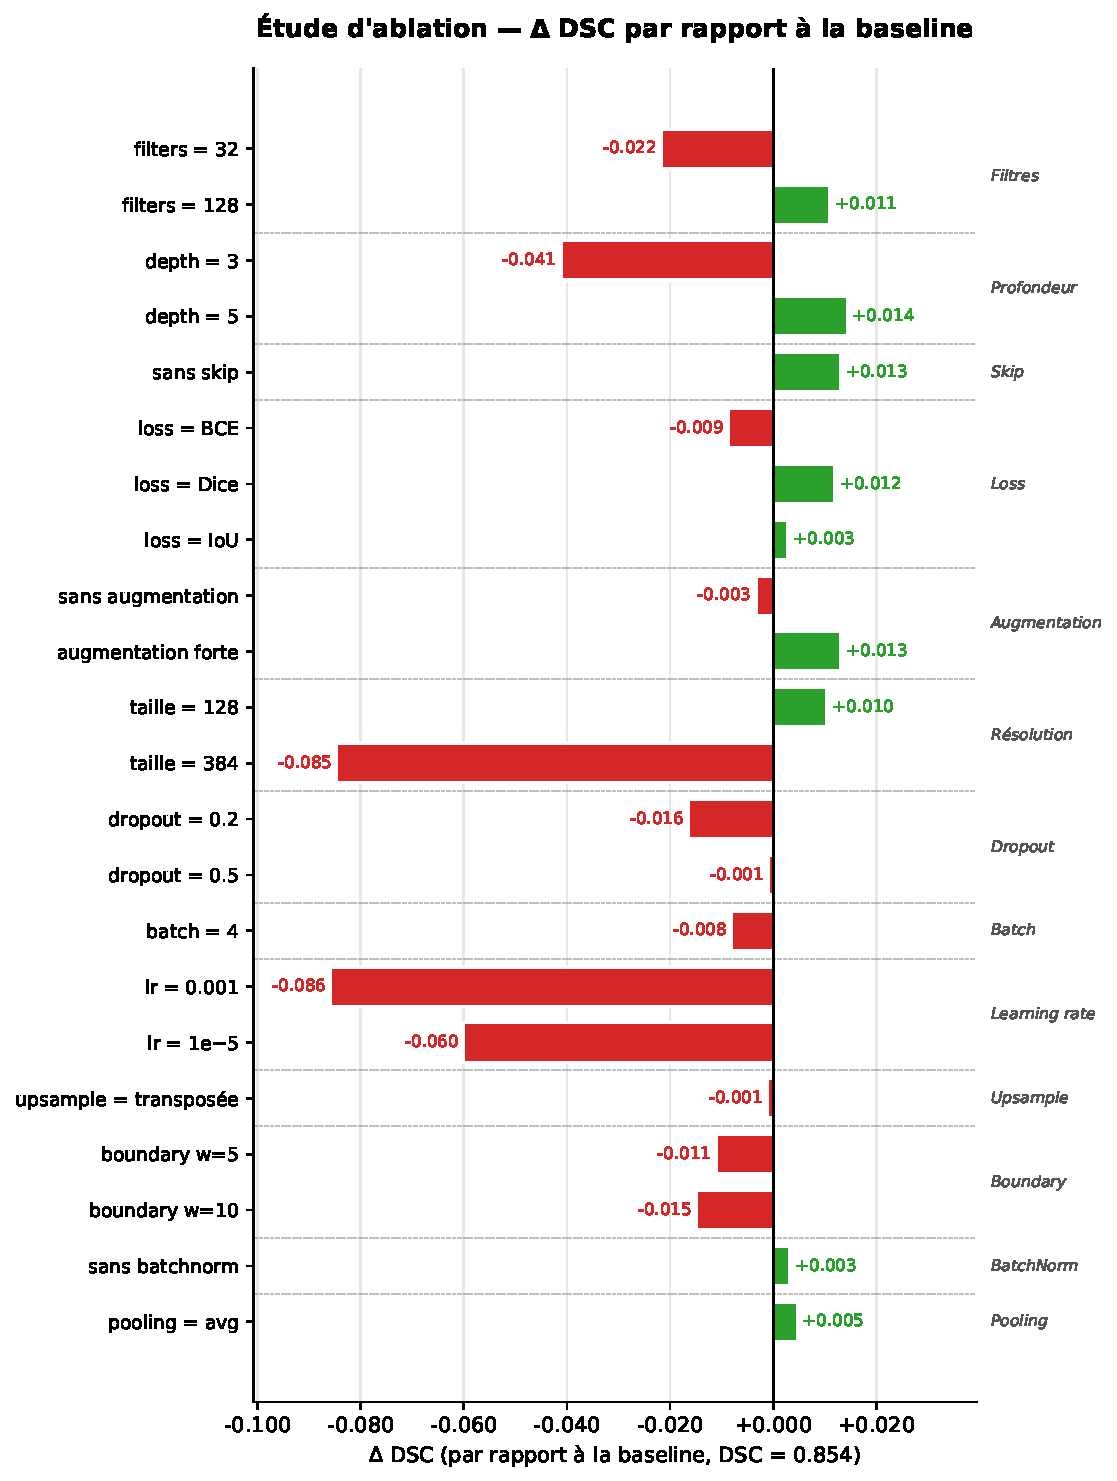
\includegraphics[width=0.85\textwidth]{fig_ablation_barplot.pdf}
\caption{Étude d'ablation~: $\Delta$DSC par rapport à la baseline (DSC~$= 0{,}854$) pour les 22 variantes explorées, groupées par axe d'hyperparamètre. Barres vertes~: amélioration~; barres rouges~: dégradation.}
\label{fig:ablation_barplot}
\end{figure}

\subsubsection{Analyse par axe}

\paragraph{Capacité du réseau (nombre de filtres).} Le doublement du nombre de filtres de base produit des gains décroissants~: le passage de 32 à 64 filtres apporte $+2{,}2$ points de DSC (0,832 $\to$ 0,854), tandis que le passage de 64 à 128 filtres n'apporte que $+1{,}1$ point (0,854 $\to$ 0,865), pour un coût en paramètres multiplié par 4 à chaque doublement (7,9M $\to$ 31,4M $\to$ 125,5M).

\paragraph{Profondeur.} L'ajout d'un niveau de profondeur (3 $\to$ 4) produit un gain substantiel de $+4{,}1$ points de DSC (0,813 $\to$ 0,854), en cohérence avec l'augmentation du champ réceptif. En revanche, le passage de 4 à 5 niveaux n'apporte que $+1{,}4$ point (0,854 $\to$ 0,868) pour un quadruplement du nombre de paramètres (31,4M $\to$ 125,8M), suggérant que la profondeur 4 offre le meilleur compromis performance/complexité pour des images de résolution $256 \times 256$.

\paragraph{Fonction de perte.} La Dice loss seule obtient les meilleures performances (DSC $= 0{,}866$, $+1{,}2$ pts vs baseline BCE+Dice), suivie de l'IoU loss (0,857). La BCE seule est la moins performante (0,845), probablement en raison de sa sensibilité au déséquilibre de classes. Ce résultat confirme l'intérêt des fonctions de perte directement optimisées sur les métriques de recouvrement pour la segmentation de lésions.

\paragraph{Skip connections.} Sur le sous-ensemble d'ablation (50\% des données), la suppression des skip connections (DSC $= 0{,}867$) améliore légèrement les performances par rapport à la baseline (0,854). Cependant, une expérience complémentaire sur l'intégralité des données d'entraînement, avec évaluation sur le test set officiel, \textbf{inverse ce résultat}~: le modèle avec skip connections obtient un DSC test de $0{,}892$, contre $0{,}877$ sans skip ($\Delta = +0{,}014$), avec 7~échecs contre 11. Le résultat de l'ablation sur 50\% était donc un artefact du sous-échantillon, et les skip connections apportent bien un gain mesurable lorsque le modèle dispose de suffisamment de données d'entraînement. Ce résultat est cohérent avec la littérature \citep{ronneberger2015unet}, qui identifie les skip connections comme un composant essentiel de l'architecture U-Net pour la préservation des détails spatiaux.

\paragraph{Taux d'apprentissage.} Le taux $\eta = 10^{-4}$ s'avère optimal (DSC $= 0{,}854$). Un taux trop élevé ($10^{-3}$) entraîne une instabilité de l'entraînement avec convergence prématurée (DSC $= 0{,}768$, early stopping à l'epoch 16). Un taux trop faible ($10^{-5}$) ralentit la convergence sans bénéfice (DSC $= 0{,}794$ après 30 epochs).

\paragraph{Augmentation de données.} L'augmentation par retournements (\emph{flip}) apporte un gain modeste de $+0{,}3$ point par rapport à l'absence d'augmentation (0,854 vs 0,851). L'augmentation \emph{heavy} (rotations, jitter photométrique) obtient un DSC de 0,867, soit $+1{,}3$ point supplémentaire, mais ce gain pourrait être attribué en partie à la régularisation implicite plutôt qu'à une meilleure couverture de l'espace des données.

\paragraph{Résolution d'entrée.} La résolution par défaut de $256 \times 256$ constitue un bon compromis. La résolution réduite $128 \times 128$ produit des résultats comparables (DSC $= 0{,}864$) avec un temps d'entraînement significativement réduit. En revanche, la résolution $384 \times 384$ avec un mini-batch de 2 (contrainte mémoire GPU) dégrade fortement les performances (DSC $= 0{,}769$). Afin de déconfondre l'effet de la résolution et celui de la taille du mini-batch, une expérience complémentaire a été menée avec \textbf{accumulation de gradients} (batch physique $= 2$, 4~étapes d'accumulation, batch effectif $= 8$). Le résultat (DSC $= 0{,}853$) est quasi identique à la baseline $256 \times 256$ (DSC $= 0{,}854$), confirmant que la dégradation observée à $384 \times 384$ était \textbf{principalement imputable à la taille du mini-batch} ($\Delta\text{DSC} = +0{,}084$ entre batch~$= 8$ et batch~$= 2$ à résolution fixée), et non à la résolution elle-même. La résolution $256 \times 256$ reste néanmoins préférable en raison d'un coût computationnel moindre pour des performances équivalentes.

\paragraph{Dropout.} L'ajout de dropout dégrade les performances dans cette configuration~: dropout $= 0{,}2$ (DSC $= 0{,}838$, $-1{,}6$ pt) et dropout $= 0{,}5$ (DSC $= 0{,}853$, $-0{,}1$ pt). Ce résultat suggère que la capacité du réseau n'est pas excédentaire pour la taille du jeu de données utilisé en ablation (50\%).

\paragraph{Normalisation par lot.} La suppression de la normalisation par lot \citep{ioffe2015batchnorm} produit un écart de $+0{,}3$ point (DSC $= 0{,}857$ vs 0,854), trop faible pour être considéré comme significatif. Ce résultat indique que la BatchNorm n'est ni indispensable ni nuisible dans cette configuration, bien que son rôle stabilisateur devienne critique en combinaison avec certaines fonctions de perte (cf.\ section~\ref{subsec:ablation_protocole}).

\paragraph{Type de pooling.} L'\emph{average pooling} surpasse le \emph{max-pooling} de $+0{,}5$ point (DSC $= 0{,}859$ vs 0,854). Cet écart, du même ordre que la variabilité inter-entraînements, est trop faible pour conclure à une supériorité significative de l'une ou l'autre méthode.

\paragraph{Pondération aux frontières.} Contrairement à l'hypothèse initiale, la pondération des pixels proches des frontières dégrade les performances~: $w = 5$ (DSC $= 0{,}843$, $-1{,}1$ pt) et $w = 10$ (DSC $= 0{,}839$, $-1{,}5$ pt). Ce résultat suggère que l'augmentation du poids des pixels de frontière, souvent bruités ou ambigus, perturbe l'optimisation plutôt qu'elle ne la guide.

\paragraph{Méthode de sur-échantillonnage et taille de mini-batch.} L'interpolation bilinéaire et la convolution transposée produisent des résultats quasi identiques (DSC $= 0{,}854$ vs $0{,}853$). La réduction de la taille de mini-batch de 8 à 4 entraîne une légère dégradation (DSC $= 0{,}846$, $-0{,}8$ pt), cohérente avec une estimation plus bruitée du gradient.

\subsection{Modèle final optimisé}
\label{subsec:final_model}

Sur la base des enseignements de l'étude d'ablation, un modèle final est entraîné en combinant les choix d'hyperparamètres les plus performants~: \texttt{base\_filters=64}, \texttt{depth=4}, \texttt{use\_skip=True}, \textbf{Dice loss}, $\eta = 10^{-4}$, augmentation par retournements, \texttt{batchnorm=True}, \texttt{pooling=max}, \texttt{dropout=0}. Ce modèle totalise 31,4M paramètres.

Le dropout n'est pas retenu dans le modèle final~: l'ablation montrait une dégradation systématique des performances (dropout $= 0{,}2$~: $-1{,}6$ pt DSC~; dropout $= 0{,}5$~: $-0{,}1$ pt), et le faible écart train/validation observé après entraînement ($\Delta \text{DSC} = 0{,}006$) confirme l'absence de sur-apprentissage, rendant toute régularisation supplémentaire inutile.

Contrairement aux expériences d'ablation, le modèle final est entraîné sur \textbf{l'intégralité des 900 images} (720 entraînement, 180 validation). Après 30 epochs de convergence, les résultats sur l'ensemble de validation sont~:
\begin{itemize}[nosep]
    \item \textbf{DSC} $= 0{,}890$~;
    \item \textbf{IoU} $= 0{,}805$~;
    \item \textbf{Pixel Accuracy} $= 0{,}944$.
\end{itemize}

L'évaluation sur le \textbf{jeu de test officiel ISBI~2016} (379 images, jamais vues pendant l'entraînement) confirme la généralisation du modèle~:
\begin{itemize}[nosep]
    \item \textbf{DSC} $= 0{,}882 \pm 0{,}130$~;
    \item \textbf{IoU} $= 0{,}807 \pm 0{,}161$~;
    \item \textbf{Pixel Accuracy} $= 0{,}940 \pm 0{,}084$.
\end{itemize}

La faible différence entre les performances de validation et de test ($\Delta\text{DSC} = -0{,}008$) confirme l'absence de sur-apprentissage et la bonne capacité de généralisation du modèle. Par rapport à la baseline (DSC test $= 0{,}863$), le modèle final obtient un gain de $\mathbf{+1{,}9}$ point de DSC et $\mathbf{+2{,}6}$ points d'IoU sur le test set, démontrant l'efficacité de l'optimisation systématique des hyperparamètres.

\paragraph{Coût computationnel.} L'entraînement du modèle final nécessite 1\,715 secondes (28,6 minutes) sur GPU Tesla T4. L'ensemble des 24 expériences d'ablation, incluant le modèle final, représente un temps de calcul cumulé d'environ 5,6 heures.

\paragraph{Courbes d'entraînement.} La figure~\ref{fig:training_curves} présente l'évolution du coefficient de Dice et de la loss au cours des 23 epochs d'entraînement du modèle final. Le faible écart entre les courbes d'entraînement et de validation ($\Delta\text{DSC} \approx 0{,}006$ en fin d'entraînement) confirme l'absence de sur-apprentissage. Le meilleur Dice de validation ($0{,}894$) est atteint à l'epoch~20, après quoi les performances se stabilisent.

\begin{figure}[H]
\centering
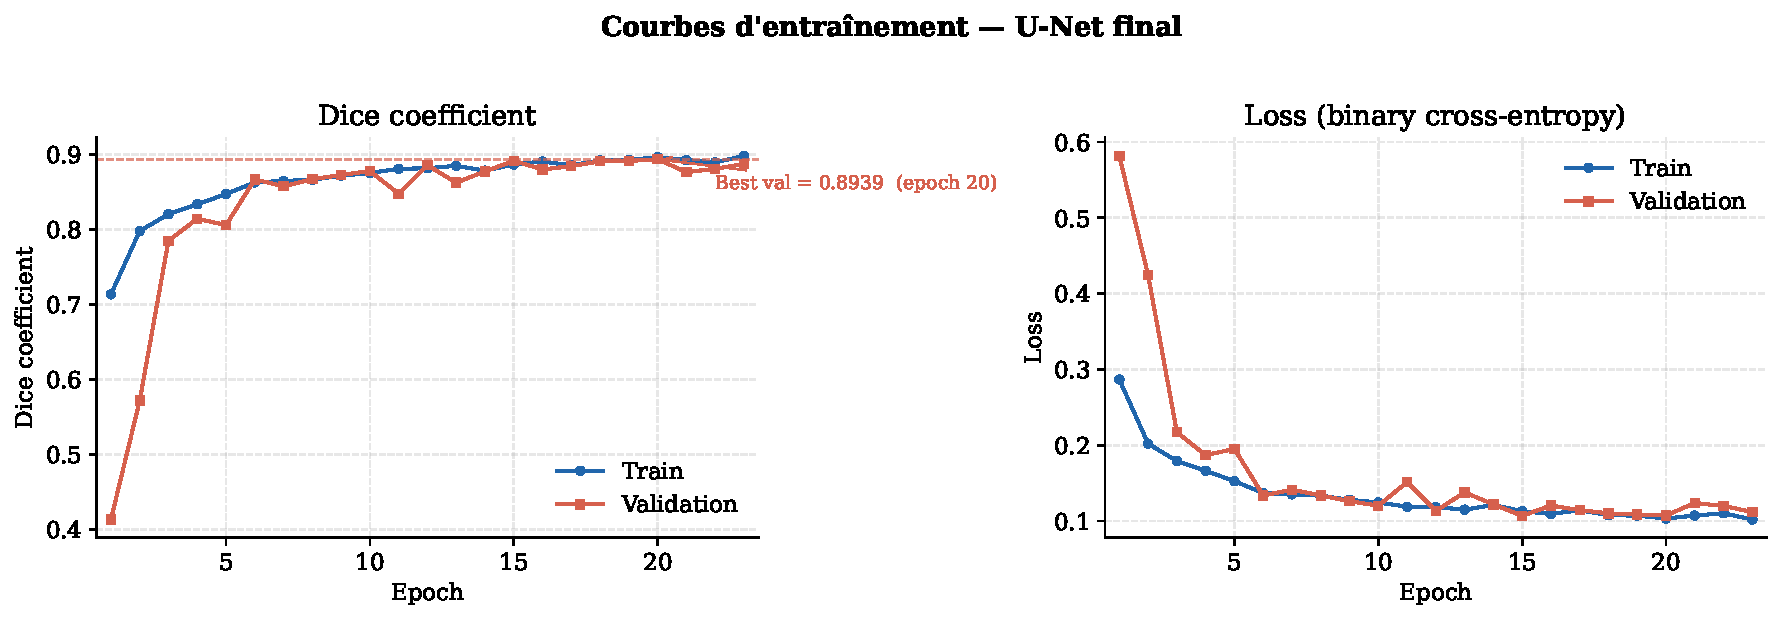
\includegraphics[width=\textwidth]{fig_unet_training_curves.pdf}
\caption{Courbes d'entraînement du U-Net final. À gauche~: coefficient de Dice (train et validation) en fonction de l'epoch. À droite~: Dice loss. La ligne horizontale pointillée indique le meilleur Dice de validation ($0{,}894$, epoch~20).}
\label{fig:training_curves}
\end{figure}

\subsection{Synthèse comparative}
\label{subsec:synthese_comparative}

Le tableau~\ref{tab:comparatif} présente la comparaison des quatre approches évaluées.

\begin{table}[H]
\centering
\caption{Comparaison des approches de segmentation sur le jeu de test officiel ISBI~2016 ($n = 379$). Toutes les métriques sont évaluées sur le même ensemble de test pour une comparaison équitable.}
\label{tab:comparatif}
\begin{tabular}{l r r r}
\toprule
\textbf{Méthode} & \textbf{DSC} & \textbf{IoU} & \textbf{Pixel Accuracy} \\
\midrule
$K$-means LAB ($K{=}2$)     & $0{,}648 \pm 0{,}346$ & $0{,}561 \pm 0{,}323$ & $0{,}840 \pm 0{,}183$ \\
CNN Patch ($P{=}32$)         & $0{,}760 \pm 0{,}175$ & $0{,}639 \pm 0{,}184$ & $0{,}868 \pm 0{,}129$ \\
U-Net baseline               & $0{,}863 \pm 0{,}143$ & $0{,}781 \pm 0{,}174$ & $0{,}932 \pm 0{,}093$ \\
\textbf{U-Net final}         & $\mathbf{0{,}882 \pm 0{,}130}$ & $\mathbf{0{,}807 \pm 0{,}161}$ & $\mathbf{0{,}940 \pm 0{,}084}$ \\
\bottomrule
\end{tabular}
\end{table}

La progression des performances, évaluées sur le même jeu de test officiel (379~images), suit fidèlement la complexité croissante des approches~: $K$-means LAB (DSC~$= 0{,}648$) $\to$ CNN patch (DSC~$= 0{,}760$, $+0{,}112$) $\to$ U-Net final (DSC~$= 0{,}882$, $+0{,}122$). Cette progression en deux étapes permet d'isoler les contributions respectives de chaque ingrédient méthodologique~:

\begin{itemize}[nosep]
    \item Le gain $K$-means $\to$ CNN patch ($+0{,}112$ DSC) est attribuable à l'introduction des \textbf{convolutions apprises} et de la \textbf{supervision}. Les features apprises sur des patches locaux surpassent les features colorimétriques brutes, même sans contexte global.
    \item Le gain CNN patch $\to$ U-Net ($+0{,}122$ DSC) est attribuable au \textbf{contexte global} et à la \textbf{cohérence spatiale}. L'architecture encodeur-décodeur avec skip connections permet de combiner détails locaux et vue d'ensemble, produisant des masques spatialement cohérents en un seul passage.
\end{itemize}

Il est important de souligner que le CNN patch, bien que supervisé, reste fondamentalement limité par son champ réceptif local ($32 \times 32$ pixels, soit 1{,}6\% de l'image). Ce modèle intermédiaire démontre que la supervision et les convolutions sont des ingrédients nécessaires mais non suffisants~: le contexte global, absent de l'approche par patches, est indispensable pour atteindre des performances de qualité clinique.

Le $K$-means conserve néanmoins un intérêt pratique dans les contextes où les annotations sont indisponibles~: sur les images à contraste élevé et sans vignettage, il atteint un DSC médian de $0{,}780$ (variante LAB), ce qui peut suffire pour un pré-criblage.

La figure~\ref{fig:comparison_qualitative} illustre cette progression sur quatre cas représentatifs du jeu de test, allant d'un cas facile (grande lésion contrastée) à un cas d'échec (petite lésion à faible contraste). On observe en particulier que le $K$-means échoue systématiquement sur les images avec vignettage (cas moyen, DSC~$= 0{,}000$), que le CNN patch produit des masques bruités aux contours irréguliers (cas difficile, DSC~$= 0{,}449$), et que le U-Net, même dans les cas difficiles, produit des segmentations spatialement cohérentes.

\begin{figure}[H]
\centering
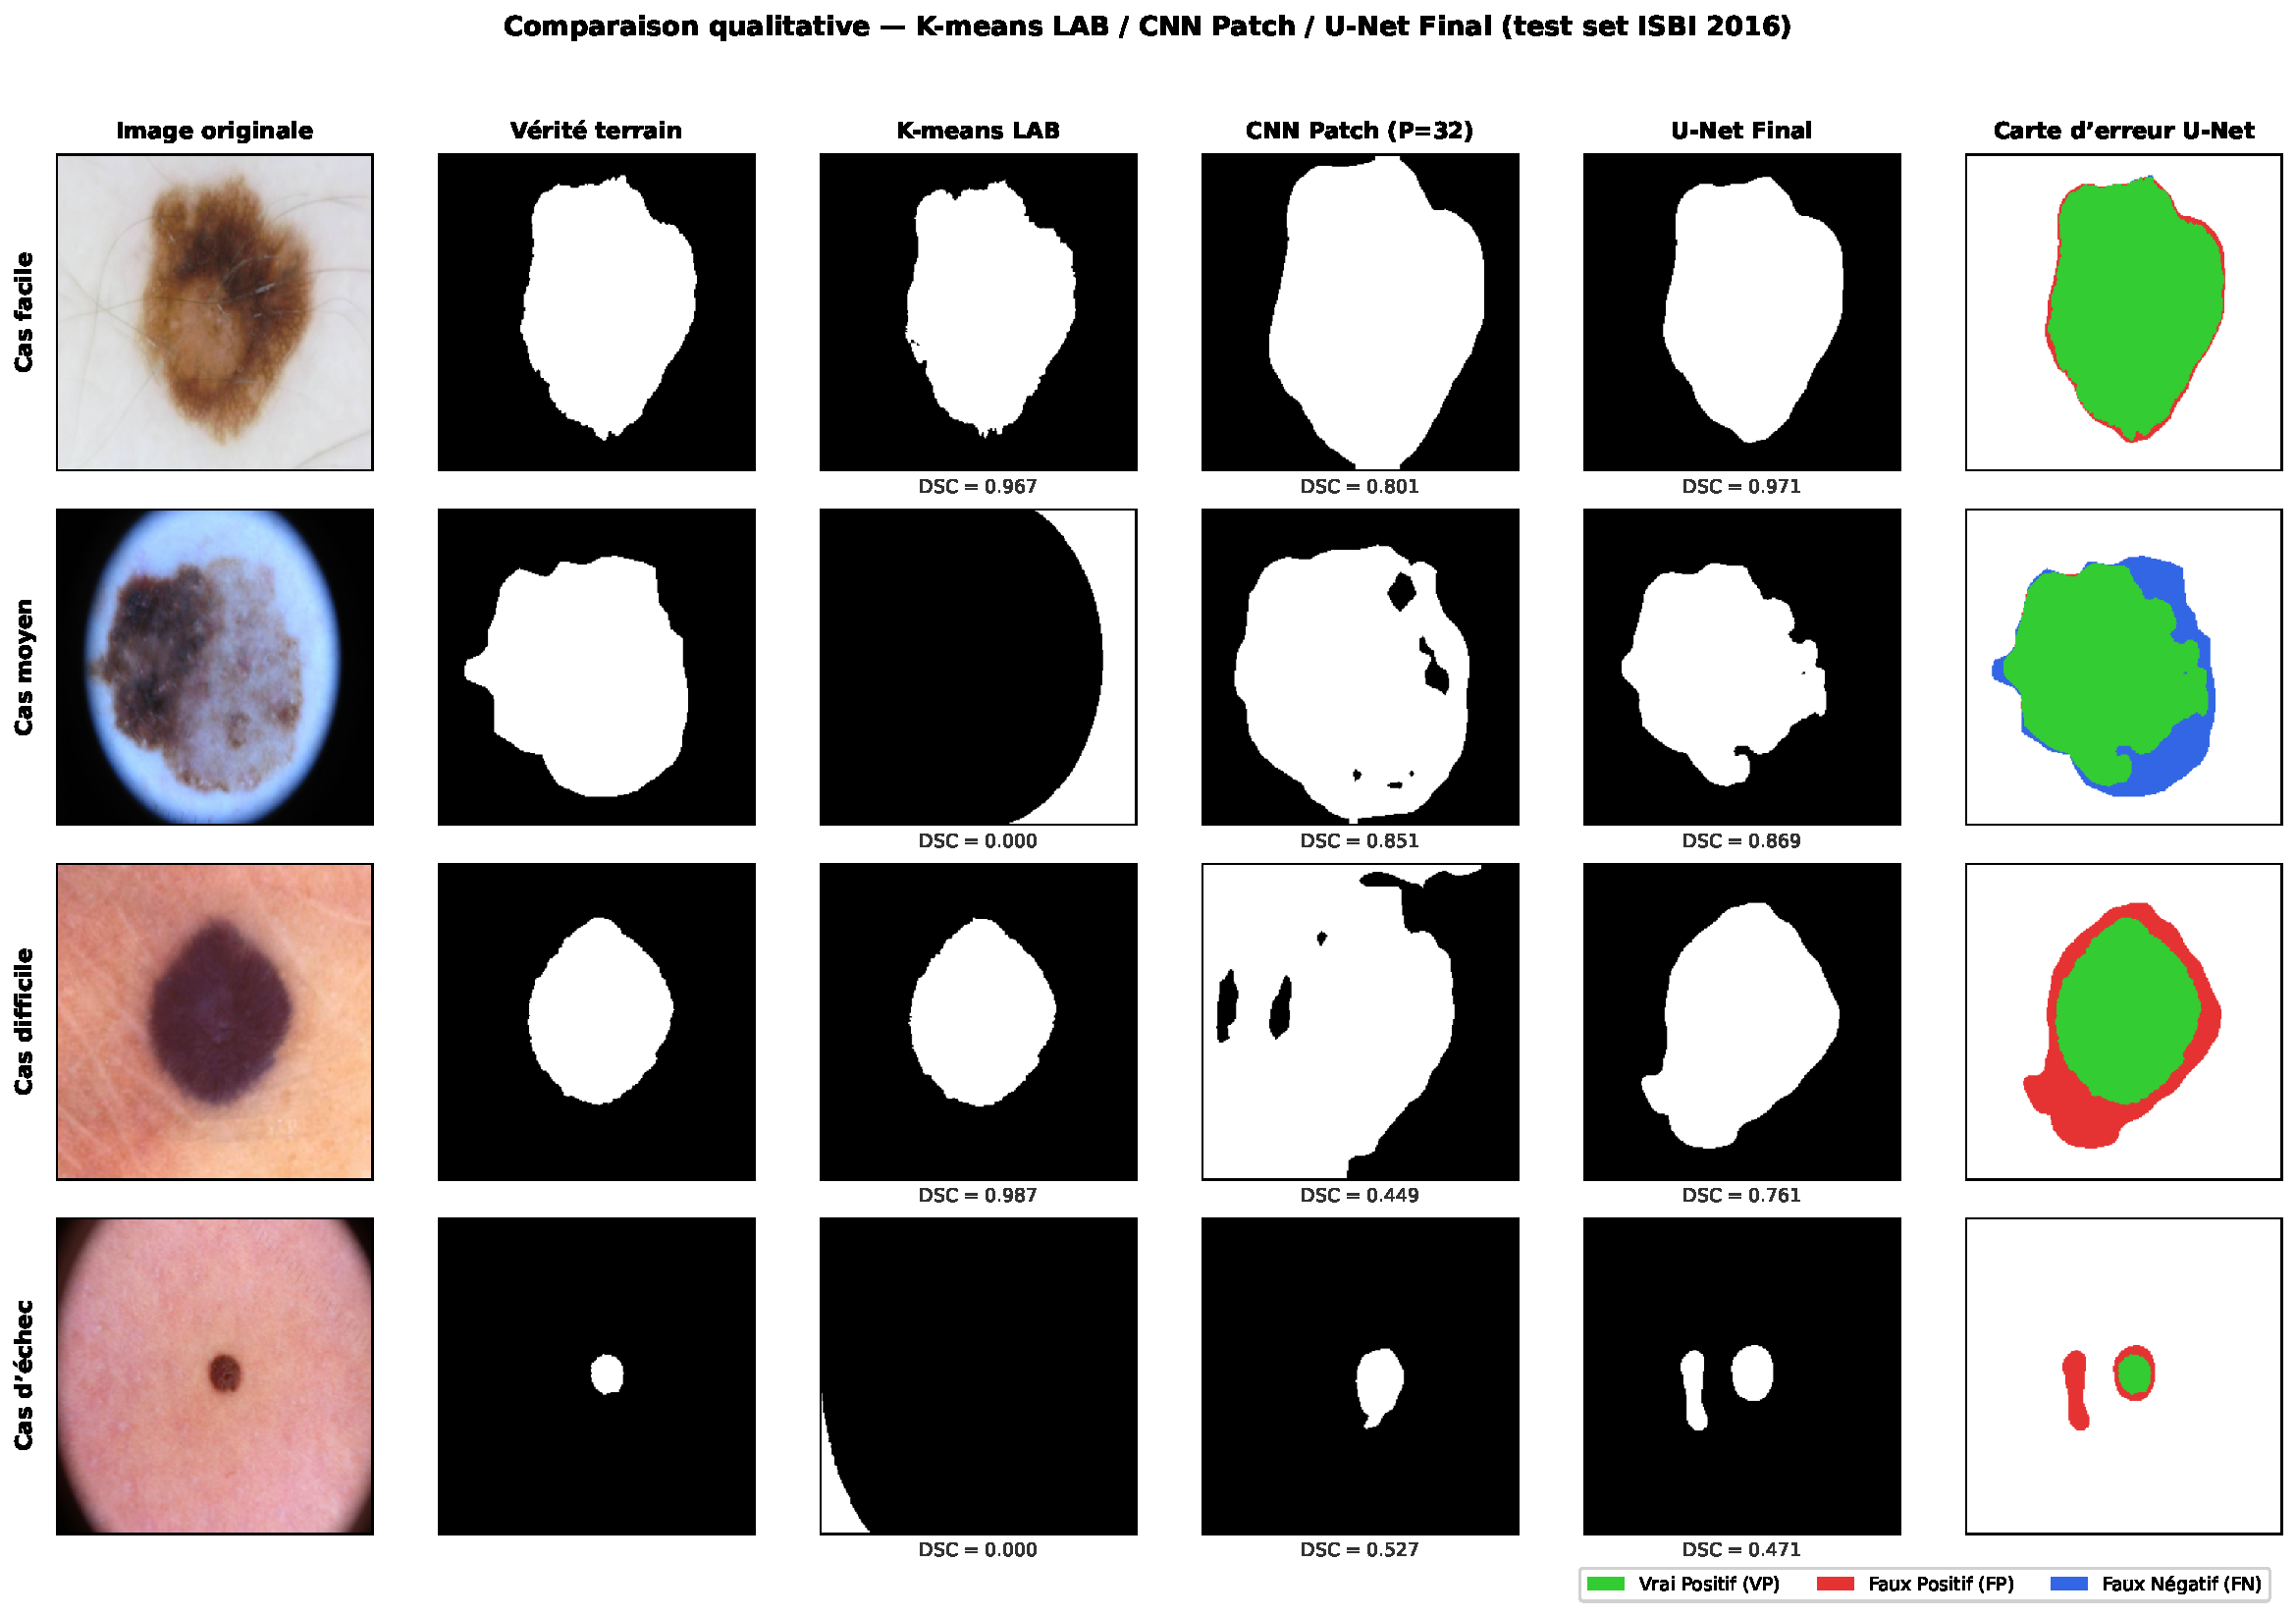
\includegraphics[width=\textwidth]{fig_comparison_qualitative.pdf}
\caption{Comparaison qualitative des trois approches sur quatre images du test set ISBI~2016, de difficulté croissante. Colonnes~: image originale, masque de référence, prédictions $K$-means LAB, CNN Patch ($P{=}32$) et U-Net Final, carte d'erreurs du U-Net (vert~= VP, rouge~= FP, bleu~= FN). Le DSC est indiqué sous chaque prédiction.}
\label{fig:comparison_qualitative}
\end{figure}

\subsubsection{Analyse par sous-groupes de taille}

Le tableau~\ref{tab:comparatif_subgroups} présente la comparaison des quatre approches par sous-groupe de taille de lésion, évaluées sur le jeu de test officiel (379~images). Cette analyse permet de mesurer la robustesse de chaque méthode face aux cas les plus difficiles.

\begin{table}[H]
\centering
\caption{Comparaison des approches par sous-groupe de taille (DSC moyen, test set ISBI~2016, $n = 379$).}
\label{tab:comparatif_subgroups}
\begin{tabular}{l r r r r r}
\toprule
\textbf{Sous-groupe} & \textbf{$n$} & \textbf{$K$-means} & \textbf{CNN Patch} & \textbf{U-Net BL} & \textbf{U-Net Final} \\
\midrule
Petites ($\rho < 5\%$)              & 40  & 0{,}197 & 0{,}590 & 0{,}708 & \textbf{0{,}719} \\
Moyennes ($5\% \leq \rho < 10\%$)   & 47  & 0{,}411 & 0{,}708 & 0{,}886 & \textbf{0{,}889} \\
Grandes ($\rho \geq 10\%$)          & 292 & 0{,}748 & 0{,}792 & 0{,}881 & \textbf{0{,}903} \\
\midrule
Global                               & 379 & 0{,}648 & 0{,}760 & 0{,}863 & \textbf{0{,}882} \\
\bottomrule
\end{tabular}
\end{table}

Deux tendances se dégagent. Premièrement, le gain apporté par la supervision est d'autant plus important que la lésion est petite~: le passage du $K$-means au U-Net final produit un gain de $+0{,}522$ DSC pour les petites lésions ($\rho < 5\%$), contre $+0{,}155$ pour les grandes ($\rho \geq 10\%$). Deuxièmement, les petites lésions restent le cas le plus difficile pour toutes les méthodes, y compris le U-Net final (DSC~$= 0{,}719$, écart-type~$= 0{,}274$), ce qui reflète la combinaison de deux facteurs~: le faible nombre de pixels informatifs et le fort déséquilibre de classes.

\subsubsection{Analyse par sous-groupes de contraste}

Le tableau~\ref{tab:comparatif_contrast} présente les performances par niveau de contraste lésion/fond $|\Delta|$, calculé comme la différence d'intensité moyenne en niveaux de gris entre les pixels de la lésion et ceux du fond (section~\ref{subsec:photometrie}).

\begin{table}[H]
\centering
\caption{Comparaison des approches par sous-groupe de contraste (DSC moyen $\pm$ écart-type, test set ISBI~2016, $n = 379$).}
\label{tab:comparatif_contrast}
\begin{tabular}{l r r r r r}
\toprule
\textbf{Contraste} & \textbf{$n$} & \textbf{$K$-means} & \textbf{CNN Patch} & \textbf{U-Net BL} & \textbf{U-Net Final} \\
\midrule
Faible ($|\Delta| < 20$)         & 74  & $0{,}320$ & $0{,}696$ & $0{,}781$ & $\mathbf{0{,}824}$ \\
Moyen ($20 \leq |\Delta| < 50$) & 138 & $0{,}596$ & $0{,}776$ & $0{,}865$ & $\mathbf{0{,}872}$ \\
Fort ($|\Delta| \geq 50$)       & 167 & $0{,}831$ & $0{,}776$ & $0{,}899$ & $\mathbf{0{,}915}$ \\
\midrule
Global                            & 379 & $0{,}646$ & $0{,}760$ & $0{,}863$ & $\mathbf{0{,}882}$ \\
\bottomrule
\end{tabular}
\end{table}

Le contraste constitue le facteur de difficulté le plus discriminant pour le $K$-means~: le DSC chute de $0{,}831$ (fort contraste) à $0{,}320$ (faible contraste), soit une dégradation de $-0{,}511$ points. Le U-Net final réduit considérablement cette sensibilité~: le DSC passe de $0{,}915$ à $0{,}824$ ($-0{,}091$ points seulement), démontrant sa capacité à exploiter la texture et le contexte spatial au-delà du seul signal d'intensité. Le gain du U-Net par rapport au $K$-means est ainsi d'autant plus marqué que le contraste est faible ($+0{,}504$ pour $|\Delta| < 20$, contre $+0{,}084$ pour $|\Delta| \geq 50$).

On note par ailleurs que le CNN patch présente un comportement atypique~: ses performances sont quasi identiques pour les contrastes moyens et forts ($0{,}776$), et inférieures au $K$-means à fort contraste ($0{,}776$ vs $0{,}831$). Ce résultat s'explique par le champ réceptif local du CNN, qui ne lui permet pas d'exploiter pleinement le contraste global de l'image.

\subsubsection{Tests de significativité statistique}

Afin de vérifier que les écarts de performance observés ne sont pas attribuables au hasard, un test de Wilcoxon \emph{signed-rank} (apparié, image par image) est appliqué aux DSC sur le jeu de test (379~images). Le tableau~\ref{tab:wilcoxon} présente les résultats.

\begin{table}[H]
\centering
\caption{Tests de Wilcoxon \emph{signed-rank} entre méthodes successives (test set, $n = 379$, bilatéral).}
\label{tab:wilcoxon}
\begin{tabular}{l r r r l}
\toprule
\textbf{Comparaison} & \textbf{$\Delta$ DSC} & \textbf{$W$} & \textbf{$p$-value} & \textbf{Sig.} \\
\midrule
CNN Patch vs $K$-means LAB       & $+0{,}115$ & 25\,439 & $3{,}0 \times 10^{-6}$  & *** \\
U-Net Baseline vs CNN Patch      & $+0{,}103$ & 11\,733 & $9{,}4 \times 10^{-30}$ & *** \\
U-Net Final vs U-Net Baseline    & $+0{,}019$ & 23\,467 & $4{,}2 \times 10^{-9}$  & *** \\
U-Net Final vs $K$-means LAB     & $+0{,}236$ & 5\,183  & $2{,}8 \times 10^{-47}$ & *** \\
\bottomrule
\end{tabular}

\smallskip
{\footnotesize ***~: $p < 0{,}001$. $\Delta$ DSC~: différence moyenne (méthode B $-$ méthode A).}
\end{table}

Toutes les comparaisons sont hautement significatives ($p < 10^{-5}$). En particulier, le gain du U-Net final par rapport à la baseline ($+0{,}019$ DSC) est modeste en valeur absolue mais statistiquement robuste ($p = 4{,}2 \times 10^{-9}$), confirmant que l'optimisation des hyperparamètres par ablation produit un gain réel et non un artefact de variance. Le gain global entre le $K$-means et le U-Net final ($+0{,}236$ DSC, $p = 2{,}8 \times 10^{-47}$) constitue la différence la plus fortement significative du jeu de comparaisons.

\subsubsection{Positionnement par rapport au challenge ISBI~2016}

Afin de situer les performances du modèle final dans le contexte de la littérature, le tableau~\ref{tab:isbi_leaderboard} compare les résultats obtenus avec les participants du challenge ISBI~2016 \citep{gutman2016isic}. Le classement officiel utilise l'indice de Jaccard (IoU) comme métrique principale.

\begin{table}[H]
\centering
\caption{Positionnement par rapport au challenge ISBI~2016 (classement officiel par Jaccard).}
\label{tab:isbi_leaderboard}
\begin{tabular}{r l l r}
\toprule
\textbf{Rang} & \textbf{Équipe} & \textbf{Méthode} & \textbf{Jaccard} \\
\midrule
1 & ExB            & Ensemble de FCN           & 0{,}843 \\
2 & CUMED          & FCRN (50+ couches)        & 0{,}829 \\
3 & Rahman         & ---                       & 0{,}822 \\
4 & sfu-mial       & CNN multi-échelle         & 0{,}811 \\
\midrule
--- & \textbf{Notre U-Net} & \textbf{U-Net (f64/d4)} & $\mathbf{0{,}807}$ \\
\midrule
6 & UiT-Seg        & ---                       & 0{,}806 \\
28 & (dernier)     & ---                       & 0{,}468 \\
\bottomrule
\end{tabular}
\end{table}

Avec un Jaccard de $0{,}807$, notre U-Net se positionnerait approximativement au \textbf{6\textsuperscript{e} rang sur 28~équipes}. Ce résultat est d'autant plus remarquable que notre architecture est un U-Net standard (31,4M paramètres) sans pré-entraînement (\emph{from scratch}), sans ensembling ni post-traitement sophistiqué, là où les équipes de tête emploient des ensembles de réseaux plus profonds (FCN, FCRN à 50+ couches). L'écart avec le premier ($\Delta\text{Jaccard} = -0{,}036$) suggère que des gains supplémentaires pourraient être obtenus via l'utilisation d'encodeurs pré-entraînés (\emph{transfer learning}) ou d'architectures plus récentes (Attention U-Net, TransUNet).

Il convient toutefois de noter que les méthodes post-challenge ont depuis largement dépassé ces résultats, atteignant des Jaccard de l'ordre de $0{,}91$ sur le même jeu de test \citep{codella2018skin}, grâce aux progrès en augmentation de données, architectures à attention et apprentissage par transfert.


% ══════════════════════════════════════════════
% 6. CONCLUSION
% ══════════════════════════════════════════════
\section{Conclusion}
\label{sec:conclusion}

Ce projet a permis d'implémenter et de comparer systématiquement trois approches de segmentation de lésions cutanées en imagerie dermoscopique, de complexité croissante, sur le jeu de données ISIC~2016.

La segmentation non supervisée par $K$-means, évaluée de manière exhaustive (quatre espaces colorimétriques, trois méthodes d'estimation du $K$ optimal, deux règles d'assignation), a établi une baseline rigoureuse (DSC~$= 0{,}648$ sur le test set) tout en mettant en évidence les limites structurelles de l'approche~: absence de modélisation spatiale (vulnérabilité au vignettage), hypothèse de clusters sphériques, et taux d'échec élevé sur les petites lésions et les images à faible contraste. L'espace CIE~LAB s'est avéré le plus performant, conformément à son uniformité perceptuelle, et l'analyse data-driven du nombre optimal de clusters a confirmé empiriquement l'adéquation de la partition binaire ($K = 2$).

Le CNN par patches (DSC~$= 0{,}760$) a démontré l'apport conjoint des convolutions apprises et de la supervision, réduisant le taux d'échec de 23{,}7\% à 7{,}7\%. Son analyse a révélé un compromis contre-intuitif entre taille de patch et performance, les petits patches ($P = 32$) surpassant les grands ($P = 64$) en raison de la dilution du signal discriminant et de la résolution de la grille d'inférence.

L'étude d'ablation du U-Net, portant sur 13 axes d'hyperparamètres et 24 expériences, a permis d'identifier les facteurs les plus influents~: la profondeur du réseau, la fonction de perte (Dice loss), et le taux d'apprentissage. Le modèle final optimisé atteint un DSC de $0{,}882 \pm 0{,}130$ et un Jaccard de $0{,}807 \pm 0{,}161$ sur le jeu de test officiel, un résultat compétitif qui se positionnerait au 6\textsuperscript{e} rang du challenge ISBI~2016 avec une architecture nettement plus simple que celles des équipes de tête.

La démarche progressive adoptée --- du $K$-means au CNN patch puis au U-Net --- a permis d'isoler les contributions de chaque ingrédient méthodologique (caractéristiques colorimétriques, convolutions apprises, supervision, contexte global, cohérence spatiale), offrant une compréhension fine des mécanismes sous-jacents aux gains de performance.


% ══════════════════════════════════════════════
% 7. PERSPECTIVES
% ══════════════════════════════════════════════
\section{Perspectives}
\label{sec:perspectives}

Plusieurs directions de recherche restent ouvertes pour prolonger ce travail~:

\begin{enumerate}
    \item \textbf{Extension multi-classes.} L'approche actuelle se limite à la segmentation binaire (lésion vs. fond). Une extension vers la classification simultanée de sous-types de lésions (mélanome, n\ae vus bénin, kératose) nécessiterait l'adaptation des fonctions de perte et des métriques d'évaluation.

    \item \textbf{Évaluation sur d'autres jeux de données.} La généralisation du modèle devrait être évaluée sur des corpus indépendants (ISIC~2017, ISIC~2018, PH$^2$) afin de mesurer sa robustesse face à des conditions d'acquisition différentes.

    \item \textbf{Architectures plus récentes.} Des variantes de U-Net intégrant des mécanismes d'attention (Attention U-Net) ou des \emph{transformers} (TransUNet) pourraient améliorer la capture des dépendances à longue portée, particulièrement utiles pour les lésions de grande taille.

    \item \textbf{Analyse d'erreurs ciblée.} L'analyse par sous-groupes de taille et de contraste réalisée dans ce travail pourrait être approfondie par une étude des cas d'échec résiduels du U-Net, en intégrant des critères supplémentaires (présence d'artefacts pileux, type de dermatoscope, morphologie des contours) afin de guider les améliorations futures.

    \item \textbf{Interprétabilité.} L'application de méthodes d'explicabilité telles que Grad-CAM \citep{selvaraju2017gradcam} permettrait de visualiser les régions de l'image les plus influentes dans la décision du modèle, renforçant la confiance des cliniciens dans les prédictions.
\end{enumerate}


% ══════════════════════════════════════════════
% BIBLIOGRAPHIE
% ══════════════════════════════════════════════
\newpage
\bibliographystyle{apalike}

\begin{thebibliography}{99}

\bibitem[Arthur \& Vassilvitskii, 2007]{arthur2007kmeans++}
Arthur, D., \& Vassilvitskii, S. (2007).
\newblock $k$-means++: The advantages of careful seeding.
\newblock \textit{Proceedings of the 18th Annual ACM-SIAM Symposium on Discrete Algorithms (SODA)}, pp.~1027--1035.

\bibitem[Codella \textit{et al.}, 2018]{codella2018skin}
Codella, N.~C.~F., Gutman, D., Celebi, M.~E., Helba, B., Marchetti, M.~A., Dusza, S.~W., \ldots\ \& Halpern, A. (2018).
\newblock Skin lesion analysis toward melanoma detection: A challenge at the 2017 International Symposium on Biomedical Imaging (ISBI).
\newblock \textit{IEEE 15th International Symposium on Biomedical Imaging (ISBI)}, pp.~168--172.

\bibitem[Ciresan \textit{et al.}, 2012]{ciresan2012deep}
Ciresan, D., Giusti, A., Gambardella, L.~M., \& Schmidhuber, J. (2012).
\newblock Deep neural networks segment neuronal membranes in electron microscopy images.
\newblock \textit{Advances in Neural Information Processing Systems (NeurIPS)}, 25, 2843--2851.

\bibitem[Dice, 1945]{dice1945measures}
Dice, L.~R. (1945).
\newblock Measures of the amount of ecologic association between species.
\newblock \textit{Ecology}, 26(3), 297--302.

\bibitem[Gutman \textit{et al.}, 2016]{gutman2016isic}
Gutman, D., Codella, N.~C.~F., Celebi, M.~E., Helba, B., Marchetti, M.~A., Mishra, N.~K., \& Halpern, A. (2016).
\newblock Skin lesion analysis toward melanoma detection: A challenge at the International Symposium on Biomedical Imaging (ISBI) 2016.
\newblock \textit{arXiv preprint arXiv:1605.01397}.

\bibitem[Hesamian \textit{et al.}, 2019]{hesamian2019deep}
Hesamian, M.~H., Jia, W., He, X., \& Kennedy, P. (2019).
\newblock Deep learning techniques for medical image segmentation: Achievements and challenges.
\newblock \textit{Journal of Digital Imaging}, 32(4), 582--596.

\bibitem[Ioffe \& Szegedy, 2015]{ioffe2015batchnorm}
Ioffe, S., \& Szegedy, C. (2015).
\newblock Batch normalization: Accelerating deep network training by reducing internal covariate shift.
\newblock \textit{Proceedings of the 32nd International Conference on Machine Learning (ICML)}, pp.~448--456.

\bibitem[Kass \textit{et al.}, 1988]{kass1988snakes}
Kass, M., Witkin, A., \& Terzopoulos, D. (1988).
\newblock Snakes: Active contour models.
\newblock \textit{International Journal of Computer Vision}, 1(4), 321--331.

\bibitem[Kingma \& Ba, 2015]{kingma2015adam}
Kingma, D.~P., \& Ba, J. (2015).
\newblock Adam: A method for stochastic optimization.
\newblock \textit{Proceedings of the 3rd International Conference on Learning Representations (ICLR)}.

\bibitem[Liu \textit{et al.}, 2021]{liu2021review}
Liu, X., Song, L., Liu, S., \& Zhang, Y. (2021).
\newblock A review of deep-learning-based medical image segmentation methods.
\newblock \textit{Sustainability}, 13(3), 1224.

\bibitem[Long \textit{et al.}, 2015]{long2015fully}
Long, J., Shelhamer, E., \& Darrell, T. (2015).
\newblock Fully convolutional networks for semantic segmentation.
\newblock \textit{Proceedings of the IEEE Conference on Computer Vision and Pattern Recognition (CVPR)}, pp.~3431--3440.

\bibitem[MacQueen, 1967]{macqueen1967kmeans}
MacQueen, J. (1967).
\newblock Some methods for classification and analysis of multivariate observations.
\newblock \textit{Proceedings of the 5th Berkeley Symposium on Mathematical Statistics and Probability}, 1, 281--297.

\bibitem[Otsu, 1979]{otsu1979threshold}
Otsu, N. (1979).
\newblock A threshold selection method from gray-level histograms.
\newblock \textit{IEEE Transactions on Systems, Man, and Cybernetics}, 9(1), 62--66.

\bibitem[Ronneberger \textit{et al.}, 2015]{ronneberger2015unet}
Ronneberger, O., Fischer, P., \& Brox, T. (2015).
\newblock U-Net: Convolutional networks for biomedical image segmentation.
\newblock \textit{International Conference on Medical Image Computing and Computer-Assisted Intervention (MICCAI)}, pp.~234--241. Springer.

\bibitem[Selvaraju \textit{et al.}, 2017]{selvaraju2017gradcam}
Selvaraju, R.~R., Cogswell, M., Das, A., Vedantam, R., Parikh, D., \& Batra, D. (2017).
\newblock Grad-CAM: Visual explanations from deep networks via gradient-based localization.
\newblock \textit{Proceedings of the IEEE International Conference on Computer Vision (ICCV)}, pp.~618--626.

\bibitem[Siddique \textit{et al.}, 2023]{simple_unet}
Siddique, N., Paheding, S., Elkin, C.~P., \& Devabhaktuni, V. (2023).
\newblock U-Net and its variants for medical image segmentation: A review of theory and applications.
\newblock \textit{IEEE Access}, 9, 82031--82057.

\end{thebibliography}

\end{document}
